%
% Modified Friday, 11 November (KH)
%



\section{Overview of the department and its context}
\label{sec:overview}


% The School comprises around 80 staff across all categories and grades
% as well as close to 700 students ranging from undergraduates to PhD 
% students These numbers include those belonging to a number of large 
% research groups/centres in the school.
% This includes Insight whose research focus is on constraints,
% AI and data analytics
% and also includes Connect devoted to research broadly
% on networks and communication technologies. 
% These two centres account for a significant 
% proportion of the school's research students and staff.


\subsection{Provide a description of the department's structures to advance equality. This should include:}  
\instr{
\begin{itemize}
\item teaching and research focus, including discipline coverage and any areas of specialism;
\item	the total number of staff by gender and category of post; 
\item	the total number of students by programme type and gender;
\item	information on location/s.
\end{itemize}
}

\subsubsection{Teaching and research focus, including discipline coverage and any areas of specialism}



Table~\ref{tab:teachingoverview} presents an overview of the school's
main teaching activities. 
The school has strategically diversified its portfolio in the
last decade by introducing a suite of interdisciplinary programmes
(denoted \interdis)
in Data Science (BScDSA and MScDSA), Digital Humanities (BADHIT) and Psychology and Computing (BAPC), designed to increase 
student  numbers overall and  particularly to improve gender balance. 


%
% I've tried to replicate your table stye using 
% tab_taught_programes as a model
%

% Following copied verbatim down to 'end preamble'
\begin{tabbox}{!th}

\caption{Overview of the programmes on offer at CSIT}
\label{tab:teachingoverview}
\footnotesize 

\sisetup{
    group-digits=all,
    group-minimum-digits=4,
    mode=text,
    reset-text-series = false, 
    text-series-to-math = true,
    reset-text-family=false, 
    text-family-to-math=true
} % 'end preamle' marker


\begin{tabular}{P{3.8cm}
                !{\qquad}
                p{1.2cm}
                !{\quad}
                C{1.2cm}
                !{\quad}
                P{5.4cm}
                !{\qquad}
                C{1cm}
                }
\toprule

\textmd{Title}&
\textmd{Acronym}&
\makecell{First\\Intake}&
\textmd{Description}&
\makecell{Intake\\(2022)}\\ 
\midrule

BSc in Computer Science&
BScCS&
1979& 
Mainstream undergraduate CS degree 
& 85\\
\hdashline
BA in Digital Humanities and IT\interdis&
BADHIT&
2014& 
Blends IT, digital humanities and traditional arts and humanities
subjects 
&50\\
\hdashline
BSc in Data Science and Analytics\interdis& 
BScDSA&
2018&
Combines statistics and computing; focussed on data science
& 30\\
\hdashline
BA in Psychology and Computing\interdis&
BAPC&
2018& 
Degree combining psychology and  computing with an 
emphasis on human aspects of computing 
& 30\\ 
\midrule

Higher Diploma in Computer Science& 
HDACT&
1981&
Conversion programme for graduates of any
discipline & 40\\
\hdashline
MSc in Computing Science& 
MScCS&
1995& 
Advanced degree for CS graduates
&30\\
\hdashline
MSc in Interactive Media& 
MScIM&
1999&
Conversion programme for graduates of any
discipline; emphasis on IT for digital media 
&40\\
\hdashline
MSc in Data Science and Analytics\interdis& 
MScDSA&
2013&
Combines statistics and computing; focussed on data science
&30\\

% 'Postamble' material from here on also copied varbatim.
\bottomrule 
\end{tabular}



\end{tabbox}


Research in the school falls into four thematic areas:
\begin{enumerate}[noitemsep]
    \item Artificial Intelligence, Data Analytics and Algorithmics
    \item Networks, Computer Architectures and Software Systems 
    \item Interactive Media and Human Computer Interaction
    \item Security, Privacy and Ethics
\end{enumerate}

The bulk of this activity is concentrated in  research groups 
and centres such as Insight 
and Connect 
(Table~\ref{tab:researchcentres}) 
and two centres for research 
training (CRTs, see  Table~\ref{tab:crts})
hosted within the school. 

\begin{tabbox}{!t}

\caption{Funded research centres within or affiliated with the school}
\label{tab:researchcentres}
\footnotesize 

\sisetup{
    group-digits=all,
    group-minimum-digits=4,
    mode=text,
    reset-text-series = false, 
    text-series-to-math = true,
    reset-text-family=false, 
    text-family-to-math=true
}
% 'preamble ends here'

\begin{tabular}{p{2.5cm}
                p{7.5cm}
                !{\qquad}
                p{4cm}
                }
\toprule 
Name & Focus & Website\\ 

\midrule 

Insight&
Data science, analytics, and artificial intelligence, including decision optimisation & \url{https://www.insight-centre.ie}\\
\hdashline
Connect&
Future networks and communications & \url{https://connectcentre.ie/}\\
\hdashline
Enable&
Smart environments & \url{https://www.enable-research.ie/}\\
\hdashline
Confirm&
Smart manufacturing & \url{https://confirm.ie/} \\
\hdashline
Lero&
Software research, including complex
systems & \url{https://www.lero.ie}\\
\hdashline
MISL&
Networks and systems, with a focus on mobile/wireless and multimedia & \url{https://www.ucc.ie/en/misl/}\\

\bottomrule 
\end{tabular}

\end{tabbox}


\vspace{-4mm}

\begin{tabbox}{!t}

\caption[Centres for research training in the school]{Centres for research training (CRTs) in the school}
\label{tab:crts}
\footnotesize 

\sisetup{
    group-digits=all,
    group-minimum-digits=4,
    mode=text,
    reset-text-series = false, 
    text-series-to-math = true,
    reset-text-family=false, 
    text-family-to-math=true
}
\begin{tabular}{p{2.5cm}
                p{7.5cm}
                !{\qquad}
                p{4cm}
                }
\toprule
Name & Focus & Website\\ 
\midrule 

%  Lifted from 2018 Quality Review report
% Originally established by Prof. Eugene Freuder (Emeritus) as the Cork
% Constraint Computation Centre in 2001, rebranded in 2013 to Insight, the 
% SFI-funded Research Centre for data science
% & analytics, including decision optimisation. 
% Partner in the SFI-funded Confirm Research Centre for smart
% manufacturing and SFI-funded ENABLE research programme for smart
% environments. 

% Lifted from 2018 Quality Review report
% MISL (Mobile & Internet Systems Lab)
% Computer networking, especially wireless.
% Partner in the Connect SFI-funded
% Research Centre for future networks and
% the SFI-funded ENABLE research
% programme for smart environments



CRT-AI&
SFI programme to provide research training
in Artifical Intelligence;
Provides funding for 120 PhD students over four
years between 2019-2023 across five partner 
institutions. & \url{https://www.crt-ai.ie/} \\
\hdashline
Advance-CRT&
SFI programme to provide research training
on future networks and the Internet of Things with
applications for sustainable and independent living;
Provides funding for 120 PhD students over four
years between 2019-2023 across five partner 
institutions. & \url{https://www.advance-crt.ie/} \\

% Material from here on copied verbatim from model.
\bottomrule 
\end{tabular}


\end{tabbox}





\subsubsection{The total number of staff by gender and category of post}

Table~\ref{tab:headcount} provides a snapshot of staff numbers 
in the school. Professional, Managerial, and Support Staff (PMS) 
includes those in administrative roles and in IT support roles.
Researchers includes only those who conduct research; those in
research support roles are classified as PMS, as their work and
concerns align more  closely with other PMS staff. Some
have permanent PMS posts in UCC, but are acting in more senior 
roles within research centres.



% KH note on data:
% Staff data are taken from Table A of EDI spreadsheet. When classifying
% staff I have adopted two conventions:
% 1) All core IT support staff (Dave's crew) are classified as "PMS"
% 2) "Research" staff (as listed in Table A) are split
%   [a] Those who conduct research directly as classified as "research"
%        (Research Assistant, Postdoc (incl MC), Senior Postdoc,
%         Research Fellow (incl MC) and Senior Research Fellow)
%   [b] Research support staff e.g. RSOs are classified as "PMS"
% 
\begin{tabbox}{!bth}

\caption[Headcount summary of school of CSIT]{Headcount summary of CSIT (2020)
}
\label{tab:headcount}
\sisetup{
    group-digits=all,
    group-minimum-digits=4,
    group-separator = {,},
    table-format=4.1,
    mode=text,
    reset-text-series = false, 
    text-series-to-math = true,
    reset-text-family = false, 
    text-family-to-math = true
}
\footnotesize   
\begin{tabular}{p{2.5cm}
                p{7.5cm} 
                S[table-format=3.0]
                !{\qquad}
                S[table-format=2.0]
                !{\qquad}
                S[table-format=2.0\%]
                !{\qquad}
                S[table-format=2.0]} 

\toprule 
Category & Role & {M} & {F} & {F\%} & {Total}\\
\midrule 
Staff & Academics & 30 & 3 & 9\% & 33\\
\cdashline{2-6}
& Professional, Managerial, and Support (PMS) Staff\textsuperscript{1} & 13 & 12 & 48\% & 25\\
\cdashline{2-6}
& Researchers & 19 & 4 & 17\% & 23\\
\cmidrule{2-6}
& Subtotal staff & 62 & 19 & 23\% & 81\\
\midrule 
Students & Undergraduates & 390 & 121 & 24\% & 511\\
\cdashline{2-6}
& Postgraduates (taught) & 70 & 59 & 46\% & 129\\
\cdashline{2-6}
& Postgraduates (research) & 39 & 6 & 13\% & 45\\
\cmidrule{2-6}
& Subtotal students & 499 & 186 & 27\% & 685\\
\bottomrule 
\end{tabular}
{\\[.1in]
\sffamily 
\textsuperscript{1}PMS numbers include IT and research support staff.
} 
\end{tabbox}


Females are under-represented in almost all categories, particularly 
in research and  academic roles. 
The school is acutely aware of this imbalance  and it is a strategic 
priority to address this over time.
This issue and some actions to address it  are explored in Section~\ref{sec:academic}.


\subsubsection{The total number of students by programme type and gender}


Table~\ref{tab:teachingportfolio} summarises student numbers by gender. 
\ac{CS} programmes internationally have  struggled with 
under-representation of females. Gender balance tends to
be better for interdisciplinary computing programmes. 



% \khcomment{Include to indicate trajectory is upwards.}
% 

\subsubsection{Information on location(s)}

Figure~\ref{fig:wgb} shows the Western Gateway Building (WGB) on campus,
the base for all CSIT staff and most activities. Before the school was relocated to the WGB in 2009, the school was dispersed across a number of locations. The single location provides far more opportunities for interaction.

\begin{figure}[!hb]
\caption[Western Gateway Building: home to CSIT]{Western Gateway Building: home to CSIT.}
\begin{tabular}{p{7cm}p{0.4cm}p{7cm}}
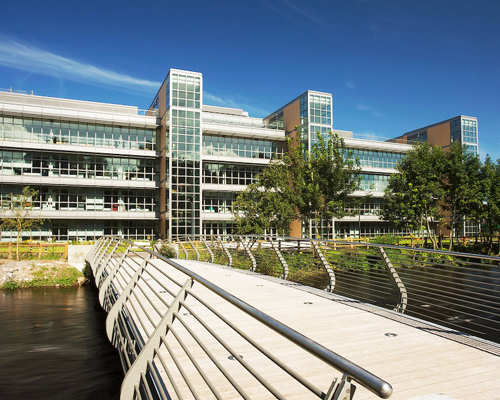
\includegraphics[align=t,height=2in]{img/WGB.jpg} 
&&
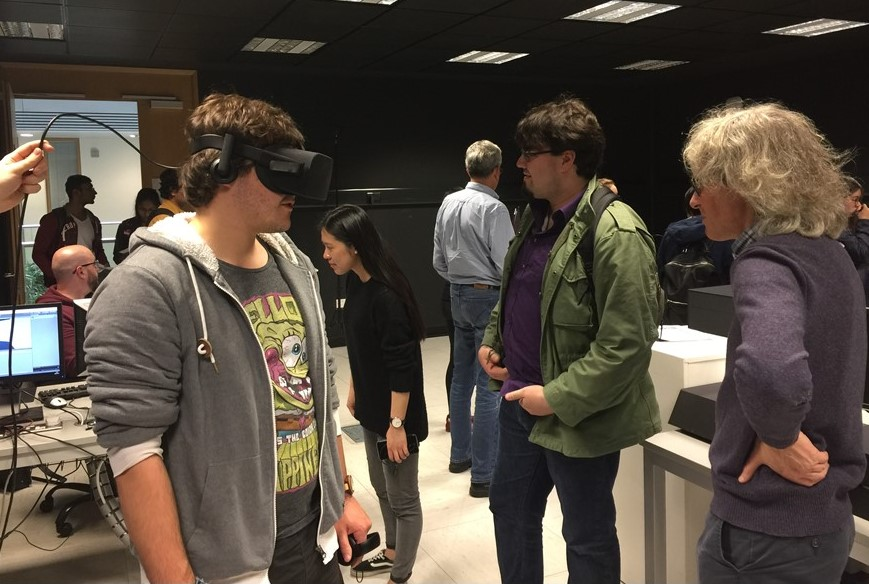
\includegraphics[align=t,height=2in]{img/vrlab.jpg}\\
\end{tabular}
\label{fig:wgb}
\end{figure}

\begin{tabbox}{!ht}

\caption[Number of students by programme and gender]{Number of students by programme and gender (2020)}
\label{tab:teachingportfolio}
\footnotesize 

\sisetup{
    group-digits=all,
    group-minimum-digits=4,
    mode=text,
    reset-text-series = false, 
    text-series-to-math = true,
    reset-text-family=false, 
    text-family-to-math=true
}
\begin{tabular}{P{4.9cm}
                !{\qquad}    
                p{6cm}
                S[table-format=3.0]
                !{\quad}
                S[table-format=2.0\%] 
                %C{3cm}
                }
\toprule 

& Programme &  {Student count} & {\% F } \\ 
\midrule
\multirow{1}{=}{Undergraduate programmes} & 
BSc in Computer Science& 299 & 14\%\\ 
\cdashline{2-4}
&BA in Digital Humanities and IT \interdis& 120 & 44\%\\ 
\cdashline{2-4}
&BSc in Data Science and Analytics \interdis&  51 & 20\% \\
\cdashline{2-4}
&BA in Psychology and Computing \interdis& 41 & 39\% \\
\cmidrule{2-4}
&Subtotal undergraduate students & 511 & 24\% \\ 

\midrule 
\multirow{1}{=}{Postgraduate taught programmes} 
& Higher Diploma  in Applied Computing&22 & 41\% \\ 
\cdashline{2-4}
& MSc in Interactive Media&38 & 68\%\\ 
 \cdashline{2-4}
& MSc in Computing Science&30 & 33\%\\
 \cdashline{2-4}
& MSc in Data Science and Analytics \interdis&39 & 36\%\\
 \cmidrule{2-4}
& Subtotal Postgraduate taught students &129 & 46\% \\ 
 
\midrule 
Postgraduate research 
& 
Postgraduate research students & 45 & 13\% \\ 

\midrule
Total student count &&  685 & 27\% \\ 
\bottomrule 
\end{tabular}
{\\[.1in]
\sffamily
Rows marked with \interdis{} indicate joint programmes with other schools.
}
\end{tabbox}




\subsection{Analyse three years of data on undergraduate students by}
\label{sec:ug_data}
\instr{
\begin{itemize}
\item gender and degree programme, with reference to discipline-specific benchmark data; 
\item gender and degree attainment;
\item gender and foundation courses.  
\end{itemize}
}

\subsubsection{Gender and degree programme, with reference to discipline-specific benchmark data}

Figure~\ref{fig:ug:enrolment} summarises three years' enrolment statistics 
by gender for our undergraduate  programmes.\footnote{BScDSA and BAPC started  in 2018-19.} The figure shows a wide variation in
female enrolment rates from 14-16\% in the BScCS
to 44-50\% in BADHIT. The former aligns better
with the school's existing research strengths, so any increase 
in female undergraduate numbers there may provide a bigger 
pool of potential research postgraduates in time.

\begin{figbox}{!ht}
    \caption{Enrolment of undergraduate students 2017-2020}
    \label{fig:ug:enrolment}
    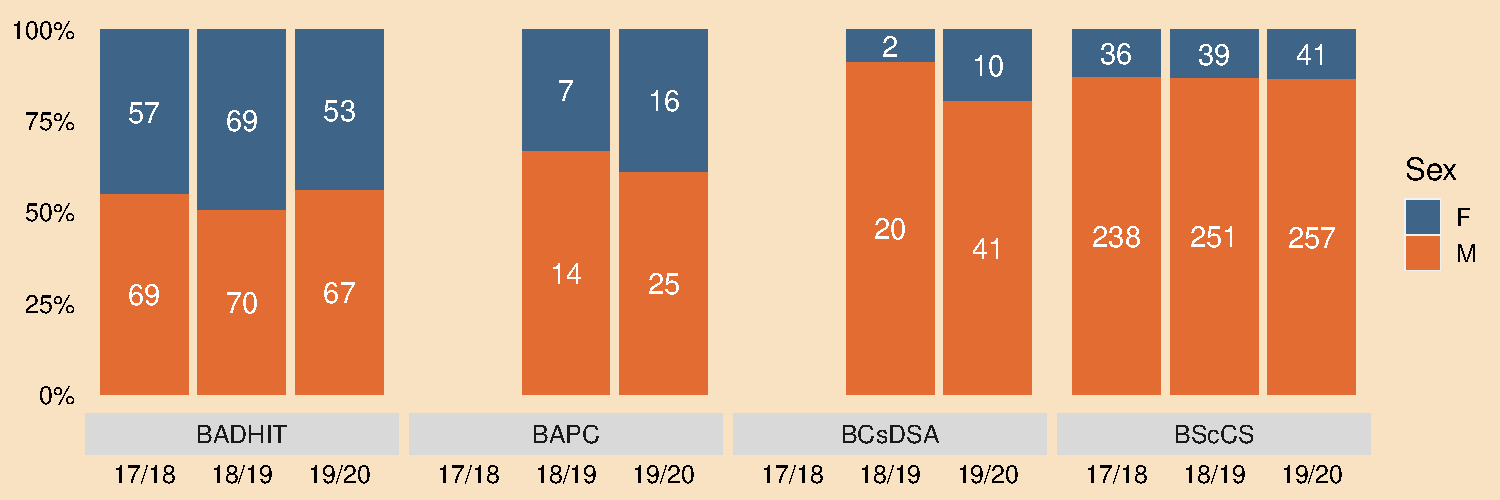
\includegraphics[width=\textwidth]{fig/ug_enrolment2.pdf}
\end{figbox}



Figure~\ref{fig:ug:mfintake} shows the evolution of the gender
breakdown linked to the introduction of new programmes
(BScDSA, BADHIT, BAPC). BADHIT and BAPC have improved 
the overall  gender balance.
In 2009-10, prior to the introduction of these newer 
programmes, the percentage of females was 14\%, compared 
with 24-25\% for the period shown.

\begin{figbox}{!t}
    \caption{Evolution of male/female intake for the BScCS programme vs. other undergraduate programmes within CSIT}
    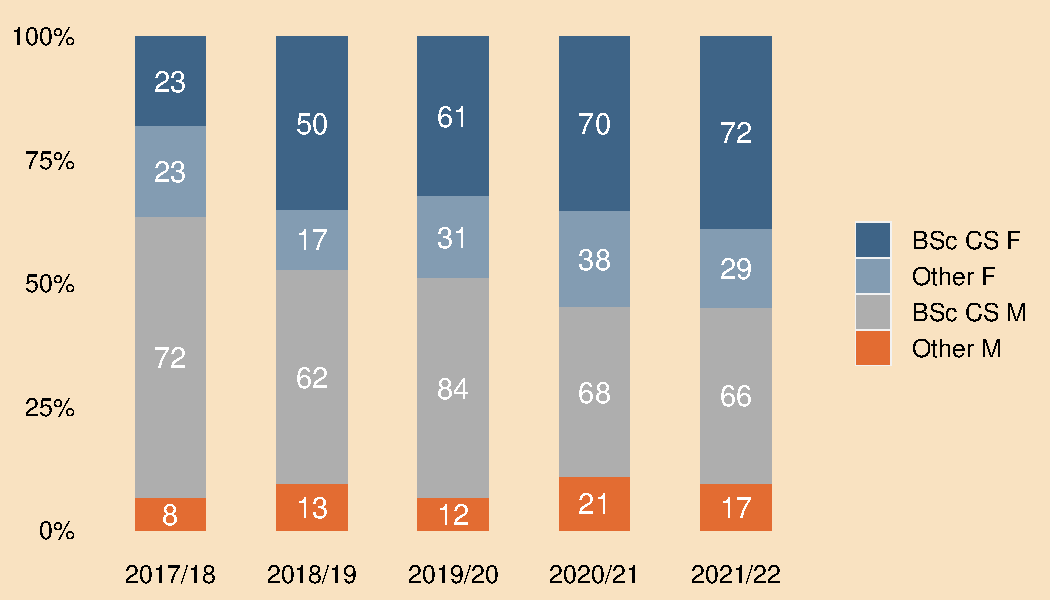
\includegraphics[width=5in]{fig/mfintake.pdf}
    \label{fig:ug:mfintake}
\end{figbox}

Table~\ref{tab:benchmarking:ug} compares CSIT's gender participation
rates for undergraduate  programmes with Irish (HEA) and UK (HESA)
benchmarks. CSIT's 22-24\% is somewhat better than the Irish (HEA) 
figure of 19-20\% and 15-16\% for the UK (HESA). 

% KH: Modified 25 October 22 to strip out raw
% numbers leaving just percentages.


\begin{tabbox}{!th}


\caption{Percentage of females on undergraduate 
programmes  for full-time students, benchmarked 
nationally (HEA) and with the 
UK (HESA)}
\label{tab:benchmarking:ug}
\footnotesize       
\sisetup{
    group-digits=all,
    group-separator = {,},
    group-minimum-digits=4,
    table-format=5.0,
    reset-text-series = false, 
    text-series-to-math = true
}
\begin{tabular}{p{2cm} 
                %S[table-format=3.1]
                %S[table-format=3.1]
                S[table-format=3.0\%]
                p{0.7cm}
                %S[table-format=3.0]
                %S[table-format=5.0]
                S[table-format=3.0\%]
                p{0.7cm}
                %S[table-format=6.0]
                %S[table-format=6.0]
                S[table-format=3.0\%]}
\toprule
Year
  & \textmd{UCC CSIT} 
  &
  &\textmd{HEA\textsuperscript{1}}
  &
  &\textmd{HESA\textsuperscript{2}}\\
%  \cmidrule{2-4}\cmidrule{6-8}\cmidrule{10-12}
 \midrule 
2017-18 &22\% && 19\% &&15\%\\
\hdashline
2018-19 &25\% &&19\% &&15\%\\
\hdashline
2019-20 &24\% &&20\% &&16\%\\ 
%   & \multicolumn{3}{c}{\textbf{UCC CSIT}} 
%   &
%   &\multicolumn{3}{c}{\textbf{HEA (Ireland)}} 
%   &
%   &\multicolumn{3}{c}{\textbf{HESA (UK)}}\\
%   \cmidrule{2-4}\cmidrule{6-8}\cmidrule{10-12}
% Year & {F}& {M} & {F\%} & & {F}& {M}& {F\%} & & {F} & {M} & {F\%}\\ 
%  \midrule 
% 2017-18 & 95  & 344 & 22\% && 908 & 3762 & 19\% && 11080 &63250 &15\%\\
% 2018-19 & 117 & 355 & 25\% && 871 & 3664 & 19\% && 11965 &65935 &15\%\\
% 2019-20 & 121 & 390 & 24\% && 910 & 3755 & 20\% && 13635 &69800 &16\%\\ 
\bottomrule 
\end{tabular}
\vspace{2mm}\\
{
\sffamily

\textsuperscript{1}\ac{HEA} percentages reflect programmes classified as \ac{ICT} 
(\ac{ISCED});\\
\textsuperscript{2}\ac{HESA} reflect programmes under heading
of Computing. 

%     The \ac{HEA} used the \ac{ISCED} and reports students studying \ac{ICT}, which % covers ICT, Database and Network 
% Design, and Software and Applications Development and Analysis. From 2019/2020 % interdisciplinary programmes 
% incorporating ICT are also included.
%     The UK \ac{HESA} \ac{HeCoS} aggregates the following subjects as Computing; % computer science, information 
%technology, information systems, software engineering, artificial intelligence, 
% computer games and animation, 
% business computing, and others in computing.

}


\end{tabbox}


\subsubsection{Undergraduate gender and degree attainment}


Figure~\ref{fig:ug:attainment} summarises the degree classifications received  
by BScCS and BADHIT graduates for the years 2018-2020. (The first graduates for 
the other two undergraduate programmes emerged only in 2021-22.)


\begin{figbox}{!t}
    \caption{Degree attainment BScCS and BADHIT}
    \label{fig:ug:attainment}
    %\includegraphics[width=\textwidth]{fig/bsc_attainment2
    \begin{subfigure}[t]{2.9in}
    \caption{Degree attainment BScCS}
    \label{fig:bsc:attainment}
    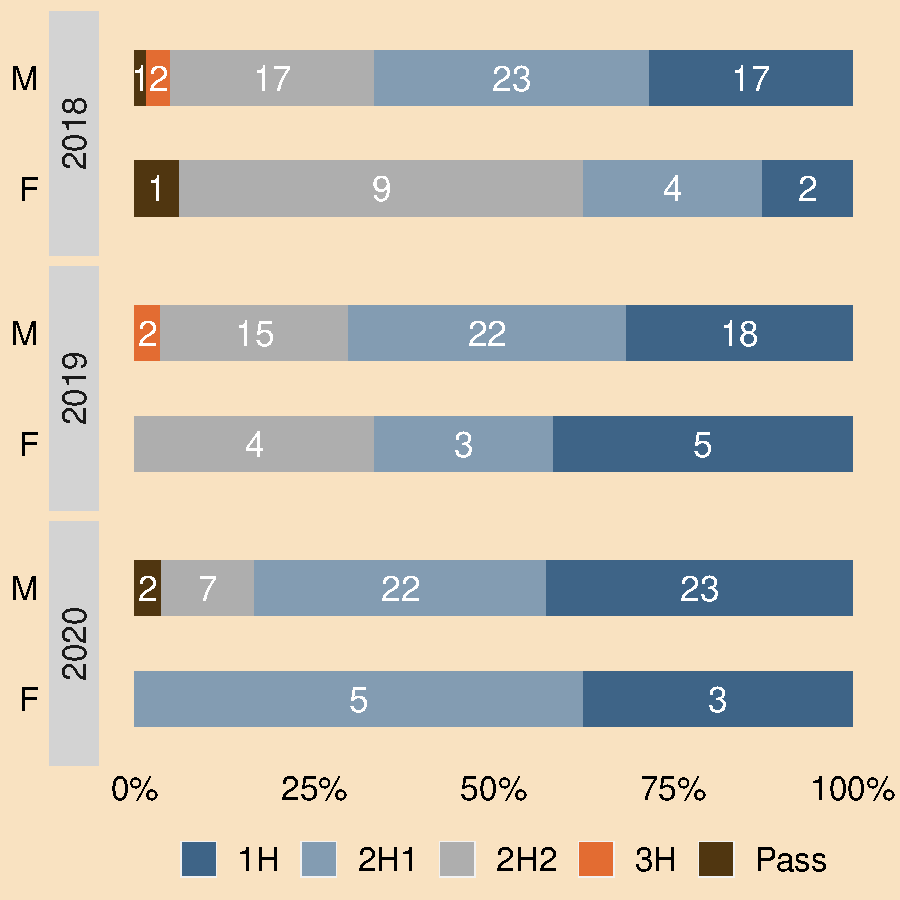
\includegraphics[width=2.8in]{fig/ug_attain2.pdf} % NEW
    \end{subfigure}
    %\includegraphics[width=4in]{fig/bsc_attainment2.pdf} %% OLD
    %
    \begin{subfigure}[t]{2.8in}
    \caption{Degree attainment BADHIT}
    \label{fig:badhit:attainment}
    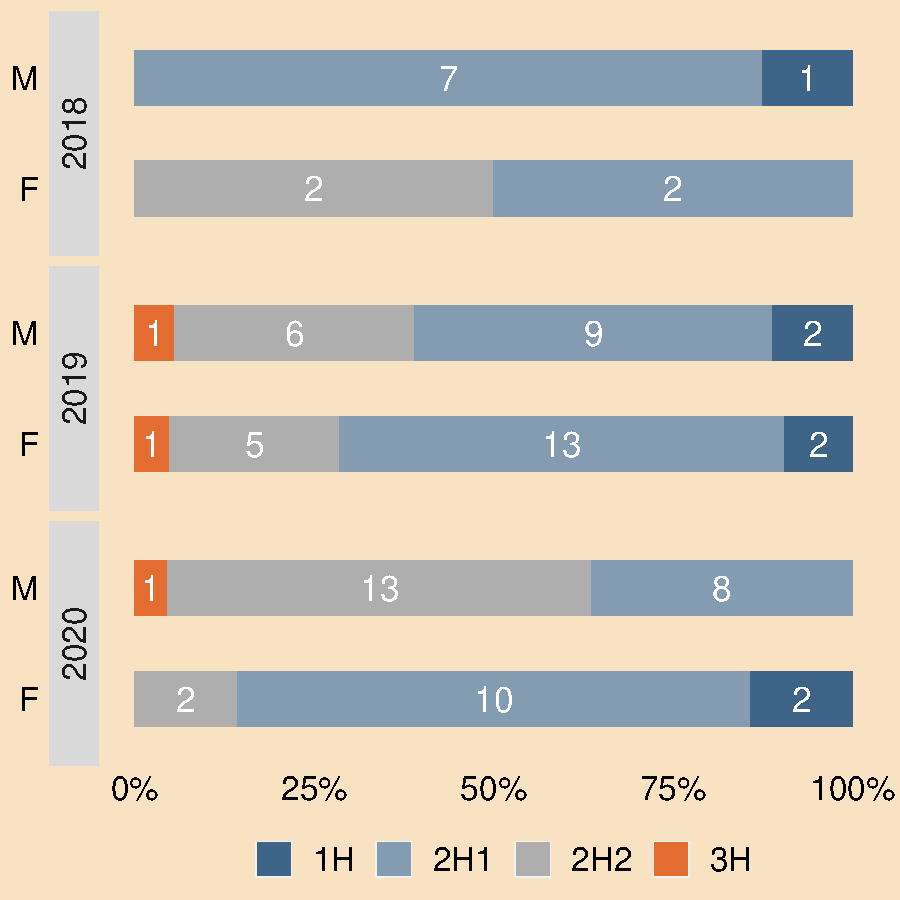
\includegraphics[width=2.8in]{fig/badhit_attainment.pdf}
    \end{subfigure}
    
\end{figbox}

Females are well represented among those  receiving higher degree classifications (Figure~\ref{fig:gradoftheyear}). The proportion of BADHIT female students receiving higher grades (2H1, 1H) was higher 
than their male classmates for two of the three years shown.
The Psychology \& Computing (BAPC) and Data Science \& Analytics (BScDSA) programmes only started in 2018; Figure~\ref{fig:ug:attainment:all} compares most recent degree attainment data across all four UG programmes.


\begin{figbox}{!t}

 \caption{Degree attainment undergraduate students across all 4 undergraduate programmes (2022)}
    %\centering
    \begin{subfigure}{2.8in}
    \caption{BScCS}
    \label{fig:attainment:bsccs}
    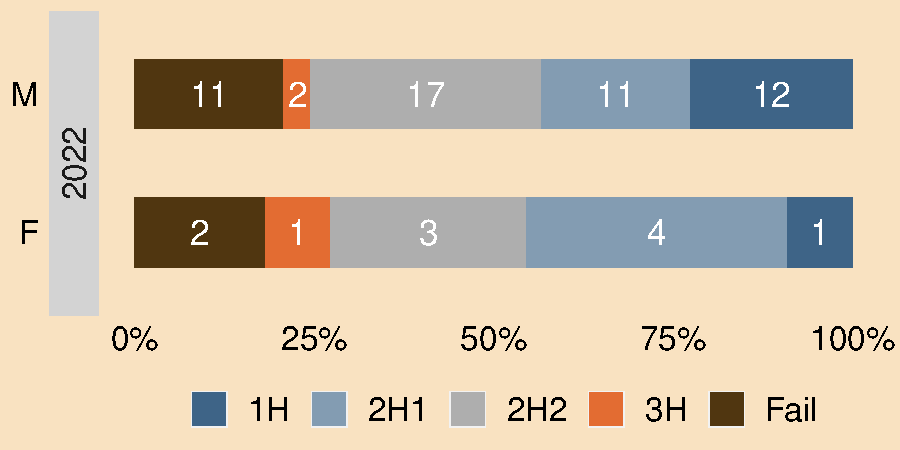
\includegraphics[width=2.8in]{fig/ug_attain_bsc22.pdf}
    \end{subfigure}
    %
    \begin{subfigure}{2.8in}
    \caption{BADHIT}
    \label{fig:attainment:badhit}
    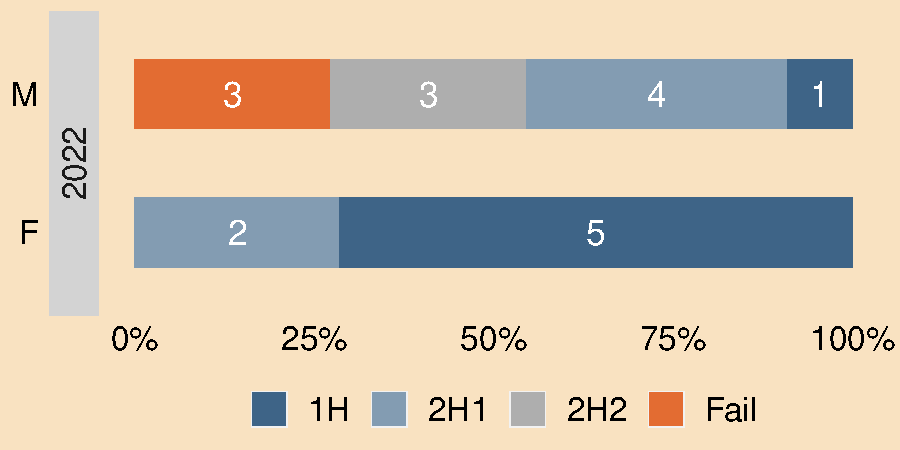
\includegraphics[width=2.8in]{fig/ug_attain_badhit22.pdf} 
    \end{subfigure}
    %
    \par\bigskip
    %
    \begin{subfigure}{2.8in}
    \caption{BAPC}
    \label{fig:attainment:bapc}
    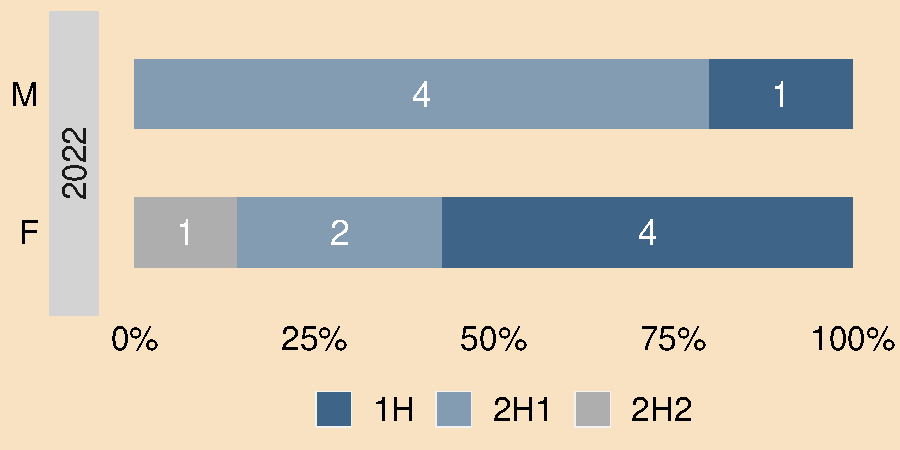
\includegraphics[width=2.7in]{fig/ug_attain_bapc22.pdf} 
    \end{subfigure}
    %
    \begin{subfigure}{2.8in}
    \caption{BScDSA}
    \label{fig:attainment:bscdsa}
    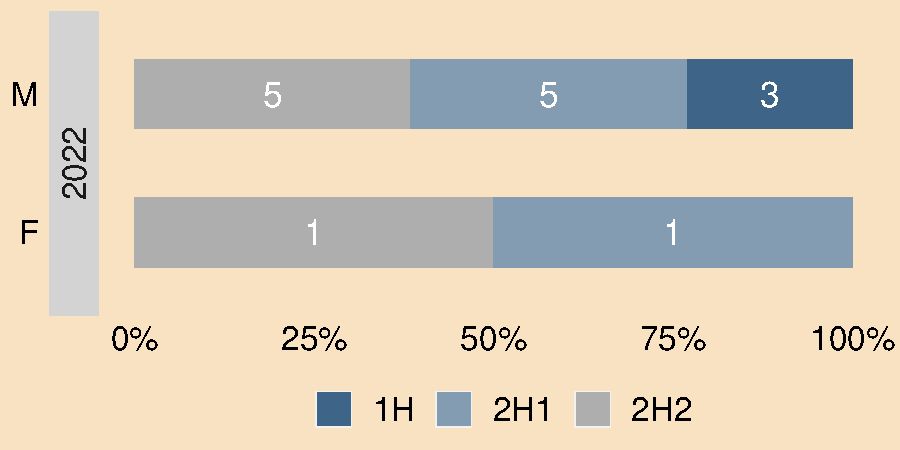
\includegraphics[width=2.7in]{fig/ug_attain_bscdsa22.pdf} 
    \end{subfigure}
    %
    \par 
    %% Add the legend
   

    
    \label{fig:ug:attainment:all}

\end{figbox}


\begin{figure}[!h]
\caption{Two CSIT undergraduate students receiving SEFS College Graduate of the Year (and runner-up) Awards.}
\label{fig:gradoftheyear}
\begin{tabular}{l !{\quad} r}
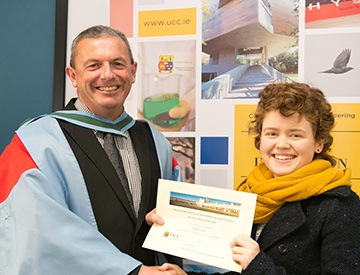
\includegraphics[height=2.15in]{img/eimearcrotty.jpg} &
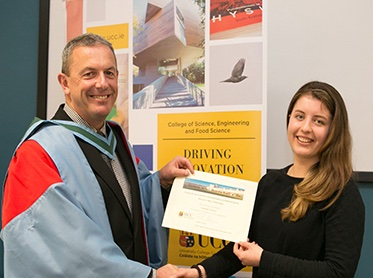
\includegraphics[height=2.15in]{img/cathbowen.jpg} \\

\end{tabular}
\end{figure}

\subsubsection{Undergraduate gender and foundation courses}

CSIT does not offer foundation courses.

\pagebreak 
\subsection{Analyse three years of data on postgraduate taught students by:} 
\instr{
\begin{itemize}
    \item gender and degree programme, with reference to discipline-specific benchmark data;  
    \item gender and degree attainment.  
\end{itemize}
}
\label{pg_data}


\subsubsection{Postgraduate taught student gender and degree programme, with reference to discipline-specific benchmark data}


Figure~\ref{fig:pg:enrolment} shows three years' enrolment data for our taught
postgraduate programmes. Female participation rates are generally better 
for postgraduate programmes than for undergraduate. The MScIM, which also attracts 
students with non-computing backgrounds, is the only programme
where females (56-68\%)  outnumber males. Both MScCS and MScDSA 
have a high proportion of non-EU students and a significantly 
better gender balance, possibly due to higher participation 
among females in STEM subjects in some non-EU countries.


\begin{figbox}{!ht}
    \caption{Enrolment postgraduate students 2017-2020}
    \label{fig:pg:enrolment}
    %\centering
    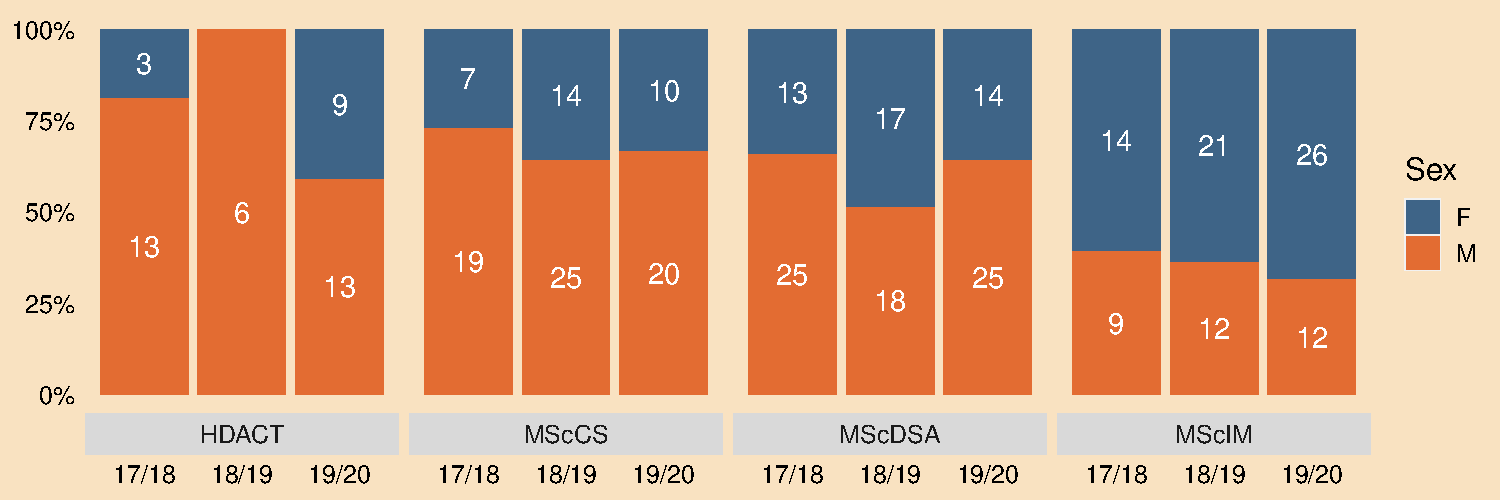
\includegraphics[width=\textwidth]{fig/pg_enrolment.pdf}
\end{figbox}


% KH: modified 25 Oct 22 to strip out raw numbers
% and leave percentages. This declutres and also 
% disguises some discrepancies.

\begin{tabbox}{!th}
      
\footnotesize       
\caption[Percentage of females on postgraduate taught programmes, benchmarked nationally
(HEA) and with the UK (HESA)]{Percentage of females on postgraduate taught programmes, benchmarked nationally
(HEA) and with the UK (HESA) (full-time students only)}
\label{tab:benchmarking:pg}

\sisetup{
    group-digits=all,
    group-minimum-digits=4,
    group-separator = {,},
    table-format=4.1,
    mode=text,
    reset-text-series = false, 
    text-series-to-math = true,
    reset-text-family = false, 
    text-family-to-math = true
}
\begin{tabular}{p{2cm} 
                %S[table-format=3.1]
                %S[table-format=3.1]
                S[table-format=3.0\%]
                p{0.7cm}
                %S[table-format=3.1]
                %S[table-format=3.1]
                S[table-format=3.0\%]
                p{0.7cm}
                %S[table-format=4.1]
                %S[table-format=5.1]
                S[table-format=3.0\%]}
\toprule
  Year
  & \textmd{UCC CSIT}
  &
  &\textmd{HEA} 
  &
  &\textmd{HESA}\\
%  \cmidrule{2-4}\cmidrule{6-8}\cmidrule{10-12}
%Year & {F}& {M} & {F\%} & & {F}& {M}& {F\%} & & {F} & {M} & {F\%}\\ 
\midrule 
2017-18 &37\% &&29\%  &&30\%\\
\hdashline
2018-19 &45\% &&32\% &&31\%\\
\hdashline
2019-20 &43\% &&32\% &&30\%\\
\bottomrule 
\end{tabular}

\end{tabbox}



Figure~\ref{fig:pg:enrolment} shows increased female enrolments in our postgraduate taught programme from  
37\% to 43\%. Table~\ref{tab:benchmarking:pg} shows  
CSIT to be higher (37-45\%) compared with national (HEA) figures and UK (HESA) 
figures of 29-32\% and 30-31\%, respectively.

\subsubsection{Postgraduate taught student gender and degree attainment}

Figure~\ref{fig:pg:attainment} plots three year's data on 
the degree classifications achieved for Postgraduate Taught (PGT) programmes; females feature prominently among those achieving
higher grades.

\begin{figbox}{!ht}

 \caption{Degree attainment postgraduate students}
    %\centering
    \begin{subfigure}{2.8in}
    \caption{Postgraduate attainment HDip ACT}
    \label{fig:hdip}
    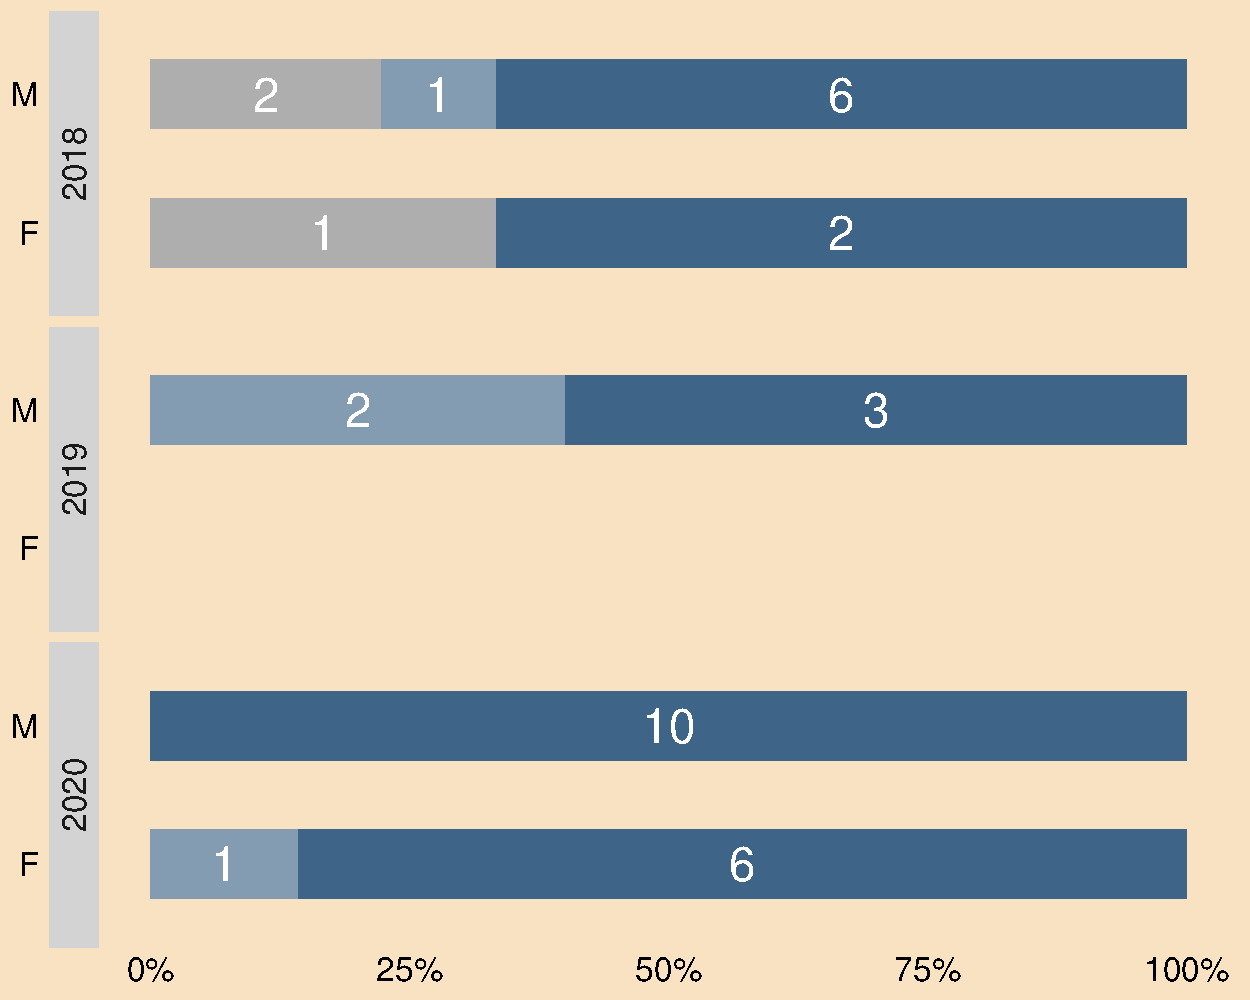
\includegraphics[width=2.8in]{fig/pg_hdact_attainment.pdf}
    \end{subfigure}
    %
    \begin{subfigure}{2.8in}
    \caption{Postgraduate attainment MSc CS}
    \label{fig:msccs}
    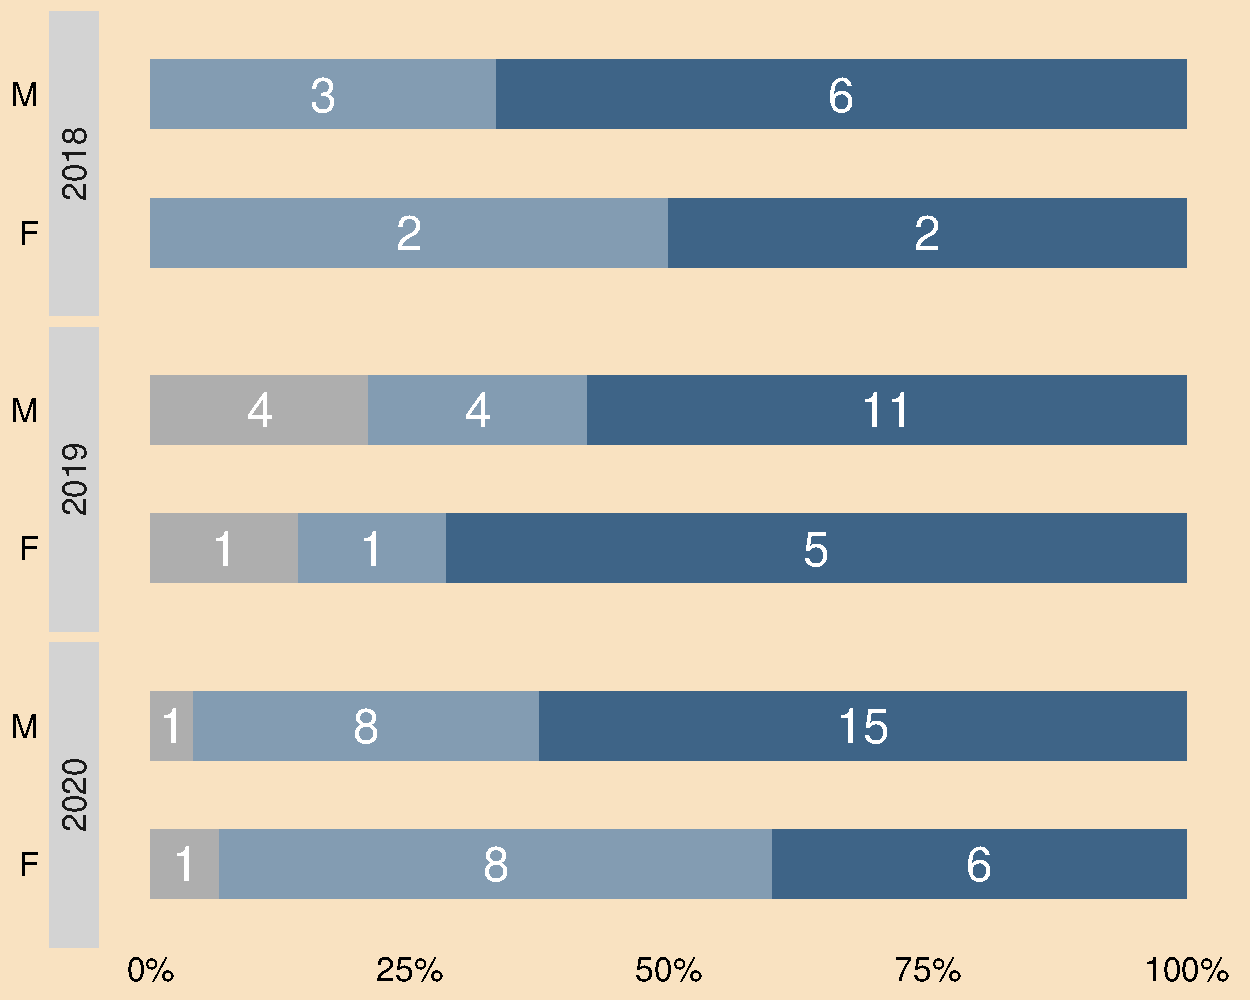
\includegraphics[width=2.8in]{fig/pg_msccs_attainment.pdf} 
    \end{subfigure}
    %
    \par\bigskip
    %
    \begin{subfigure}{2.8in}
    \caption{Postgraduate attainment MSc DSA}
    \label{fig:mscdsa}
    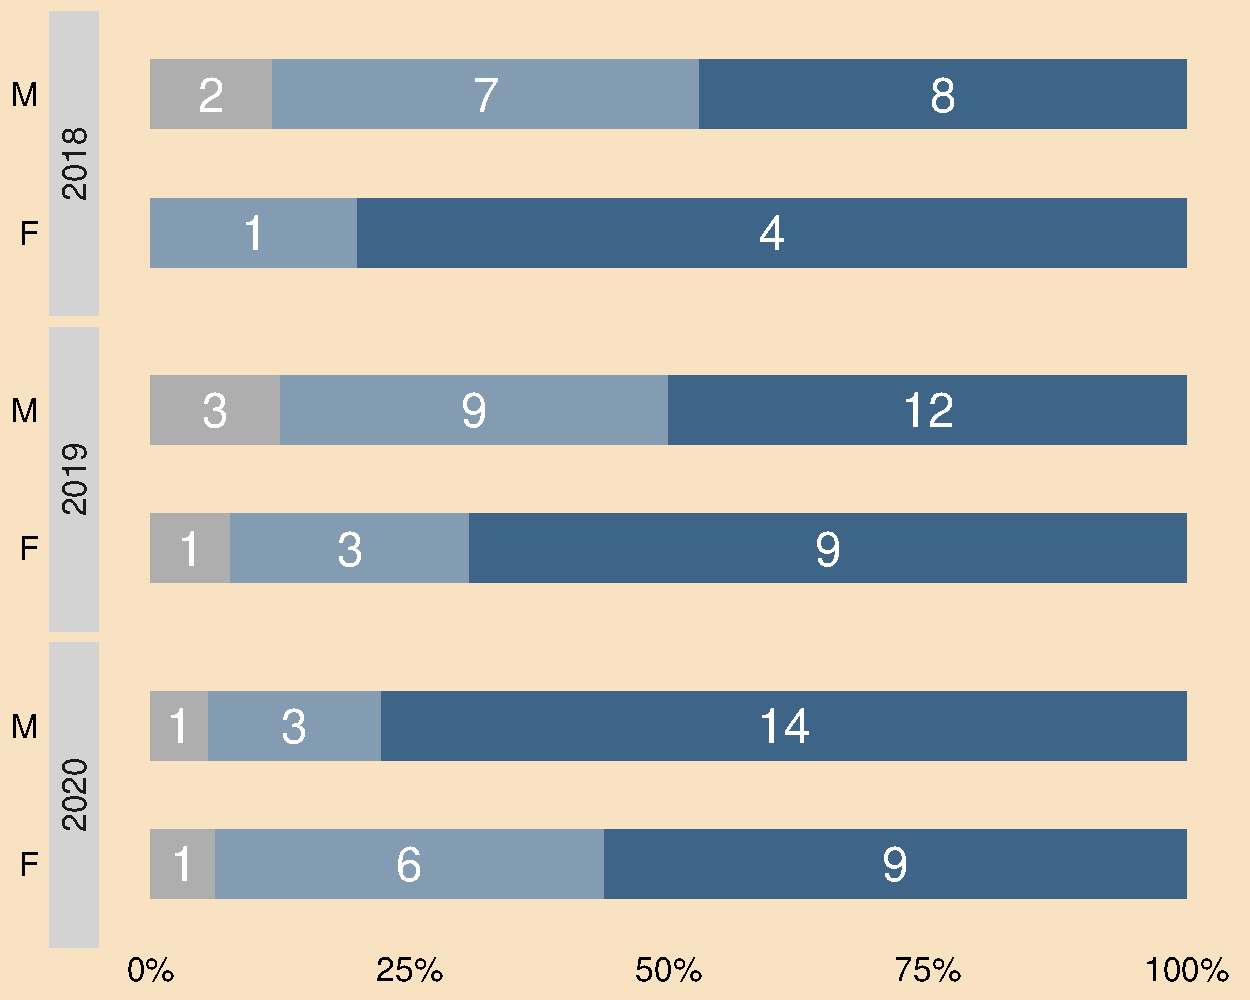
\includegraphics[width=2.7in]{fig/pg_mscdsa_attainment.pdf} 
    \end{subfigure}
    %
    \begin{subfigure}{2.8in}
    \caption{Postgraduate attainment MSc IM}
    \label{fig:mscim}
    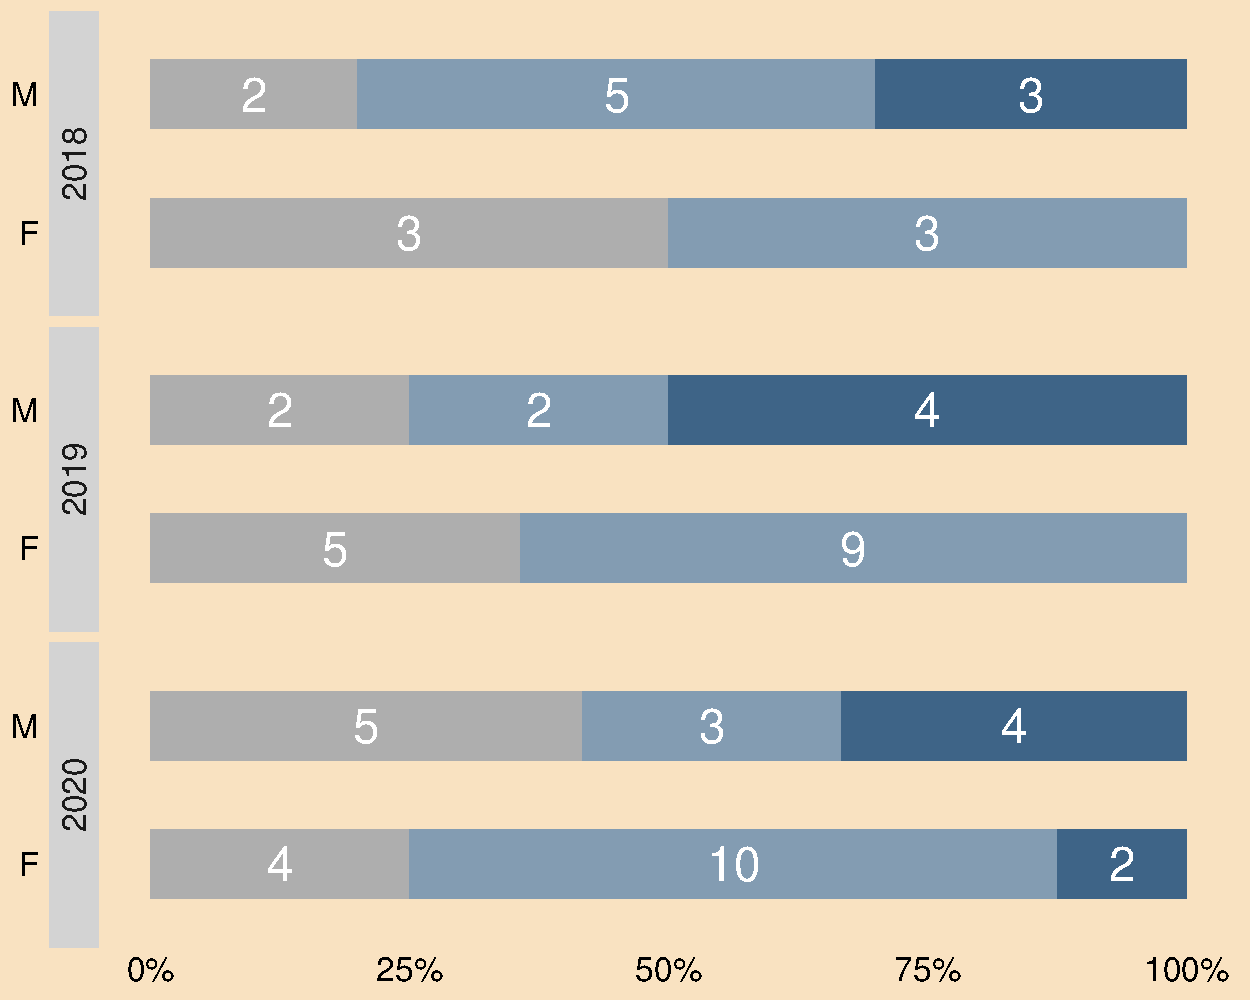
\includegraphics[width=2.7in]{fig/pg_mscim_attainment.pdf} 
    \end{subfigure}
    %
    \par 
    %% Add the legend
   
    \begin{subfigure}{14cm}
    \centering 
    % left bottom right top
    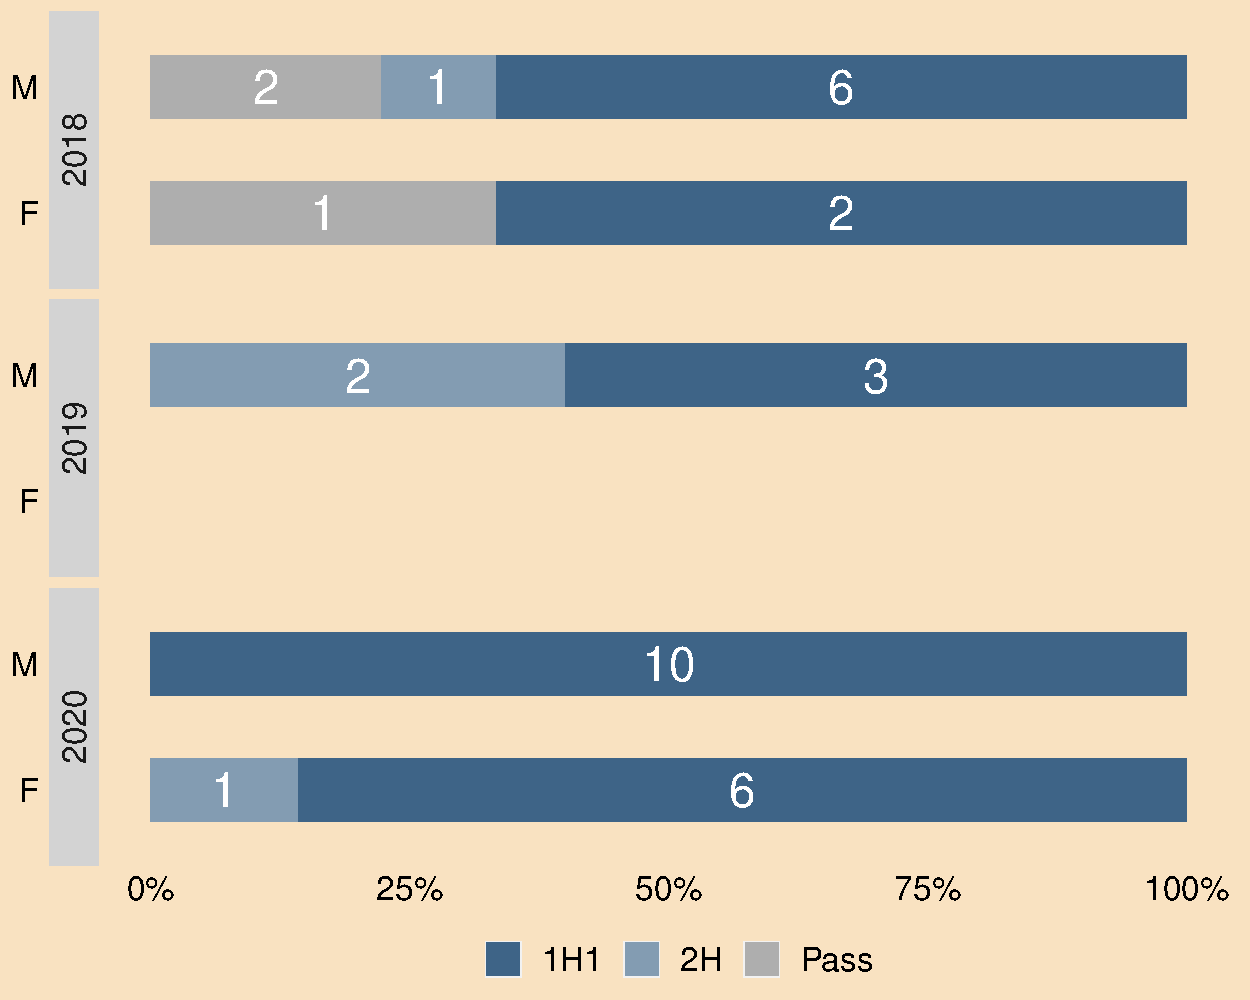
\includegraphics[trim={0 0 0 15.5cm},clip,scale=0.6]{fig/pg_legend.pdf} 
    \end{subfigure}
    
    \label{fig:pg:attainment}

\end{figbox}


\subsection{Analyse three years of data on postgraduate research 
students by:}  
\instr{
\begin{itemize}
    \item gender and enrolment; 
    \item gender and application, offer, and enrolment, with comment on how this data is collected and evaluated by the department, and on any gender disparities in student funding;  
    \item gender and completion rates.  
\end{itemize}
}
\label{sec:phdstudents}


\subsubsection{Postgraduate research student gender and enrolment}
\label{sub:phdnumbers}


Table~\ref{tab:phdregistrations} shows three years' data 
on postgraduate research students (virtually all PhDs). 
The dip in 2019-20 reflects the absence of funding before
the start of the CRTs.
%the ending of one funding source,
%before the start of the two Centres for Research Training (CRT). 
CRTs have explicit targets to 
increase female students (40\%) (Table~\ref{tab:phdintakerecent}). The percentage of females
among Postgraduate Research (PGR) students is significantly above that of the 
undergraduate population.
As SFI has gender targets attached to other funding, a similar 
pattern is expected among the non-CRT PGR intake in future years.



\input{tables2/tab_pgr_registrations_30nov}


\begin{tabbox}[7.5cm]{!th}
\caption{Postgraduate student intake since 2019-20}
\label{tab:phdintakerecent}
\footnotesize 

\sisetup{
    group-digits=all,
    group-minimum-digits=4,
    table-format=2.1,
    mode=text,
    reset-text-series = false, 
    text-series-to-math = true,
    reset-text-family=false, 
    text-family-to-math=true
}

\begin{tabular}{p{3cm}
                R{1cm}
                C{1.2cm}           
                C{1.3cm}
                R{1cm}
                }
\toprule
Year & {M} & {F} & {Total} & {\%F} \\
\midrule
2019-20 & 15 & 4 & 19 & 21\%\\
\hdashline
2020-21 & 13 & 9 & 22 & 41\%\\
\hdashline
2021-22 &  5 & 6 & 11 & 55\%\\
\bottomrule 
\end{tabular}


\end{tabbox}


A snapshot of PhD intake  by research centre or 
CRT for 2022-23 is 
shown in Table~\ref{tab:phdregistrations2223}, indicating that gender balance is improving. Figure~\ref{fig:advance:cohort} shows the 2019 cohort of ADVANCE-CRT.

\input{tables2/tab_pgr_registrations_22_23_30nov}

\begin{figure}[!t]
\caption{ADVANCE-CRT cohort 2019}
\label{fig:advance:cohort}
\begin{tabular}{c !{\quad} c}
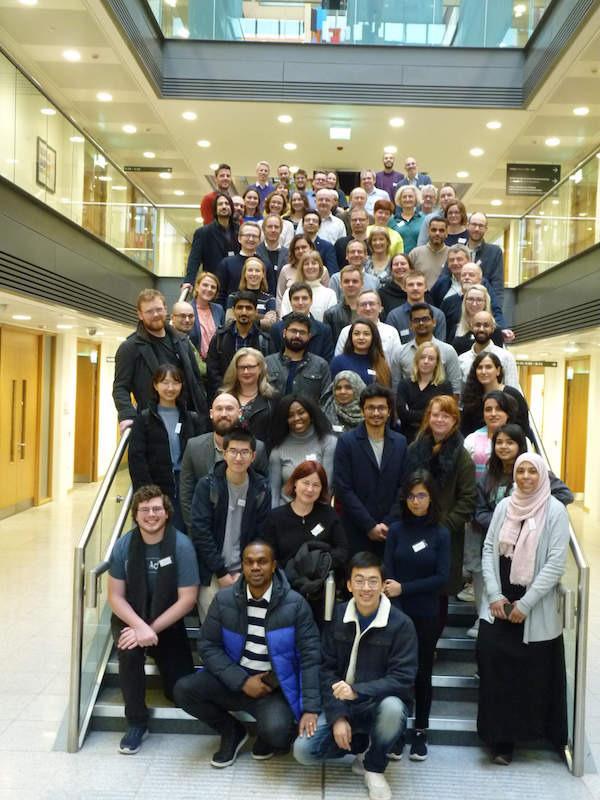
\includegraphics[width=3.6in]{img/Advance.JPG} &
\end{tabular}
\end{figure}

\subsubsection{Postgraduate research student gender and application, offer, and enrolment, with comment on how this data is collected and evaluated by the department, and on any gender disparities in student funding}
\label{sec:phdnumbers}


Historically, the PGR application process was handled by individual 
centres or PIs who maintain local 
records (see below). There has been no school-level  monitoring of number of applicants, offers 
and acceptances by gender. PGR application data will be collated under
Action~\ref{action:record:hiring:phd}.

\begin{actionblock}{\ksspace{}Collate postgraduate research application aata}{record:hiring:phd}
\acttrackgenderinfophd
\hfill{
\hypersetup{hidelinks}
\hyperlink{aa0}{\gotoactionsymbol{}
}}
\end{actionblock}

Table~\ref{tab:crtapplications} summarises the
number of applications and enrolments by gender for the two CRTs
since their introduction in 2019. 
The strategy of a quota of 40\% female enrolments has by and large been achieved in the CRTs.


\begin{tabbox}{!h}

\caption{CRT data on applications and enrolments by gender}
\label{tab:crtapplications}
\footnotesize 

\sisetup{
    group-digits=all,
    group-minimum-digits=4,
    mode=text,
    reset-text-series = false, 
    text-series-to-math = true,
    reset-text-family=false, 
    text-family-to-math=true
}
\begin{tabular}{p{3.3cm}
                p{2cm}
                C{1cm}C{1cm}C{1cm}
                C{1cm}C{1cm}C{1cm}
                C{1cm}C{1cm}C{1cm}
               }
\toprule 
&& \multicolumn{6}{c}{National} & \multicolumn{3}{c}{UCC}\\
\cmidrule(l){3-8}\cmidrule(l){9-11}
& & \multicolumn{3}{c}{Applications} 
    &\multicolumn{3}{c}{Enrolments} &\multicolumn{3}{c}{Enrolments}\\
    \cmidrule(l){3-5}\cmidrule(l){6-8}\cmidrule(l){9-11}
Centre & Year & M & F & F\% & M & F & F\% & M & F & F\% \\
\midrule


CRT-AI & 2019 &145 &89 &38\% &17 &14 &45\% &3 &1& 25\%\\
\cdashline{2-11}
& 2020 &245 &110 &31\% &15 &16 &50\% &3 &1& 25\%\\
\cdashline{2-11}
&2021 &175 &65 &27\% &14 &9 &39\% &2 &2& 50\%\\
\hdashline
ADVANCE-CRT & 2019 &162 &54 &25\% &15 &7 & 32\%& 3&2 & 40\%\\
\cdashline{2-11}
&2020 &390 &139 &26\% &9 &10 &53\% &6 &4 & 40\%\\
\cdashline{2-11}
&2021 &291 &135 &31\% &16 &13 &45\%&2 &2 & 50\%\\
\bottomrule
\end{tabular}
{\\[.1in]
\sffamily 
The application process for CRTs is handled at consortium level and students are matched with specific institutions and supervisors. Hence, it is not possible to disaggregate applications by institution.
}
\end{tabbox}







\subsubsection{Postgraduate research student gender and completion rates}

Table~\ref{tab:phdcompletionstats} shows data on
PhD completions (30\% female);
%and Table~\ref{tab:phdcompletionrates} shows 
%the completion rates (27\% female) for those expected to finish during 
%the three-years 2017-18 to 2019-20, assuming fours years to complete.
%Table~\ref{tab:phdcompletionstats} 
data were derived from
registration and graduation data.  
These figures may overstate completion 
times due to the
lag between ``finishing up'' (\emph{viva voce}, submission) 
and graduation.

\begin{tabbox}{!th}
\caption{Number of PhD graduations and average completion
times by gender for 2017-18 to 2019-20}
\label{tab:phdcompletionstats}
\footnotesize 

\sisetup{
    group-digits=all,
    group-minimum-digits=4,
    mode=text,
    reset-text-series = false, 
    text-series-to-math = true,
    reset-text-family=false, 
    text-family-to-math=true
}
\begin{tabular}{p{3.9cm}
                C{1cm}
                !{\quad}
                C{3.5cm}
                p{0.8cm}
                C{1cm}
                !{\quad}
                C{3.5cm}
               }
\toprule
& 
\multicolumn{2}{c}{Male}&&
\multicolumn{2}{c}{Female}\\
\cmidrule{2-3}\cmidrule{5-6}
Academic Year& 
Count & \makecell{Average completion\\time in months} && Count & {\makecell{Average completion\\ time in months}} \\
\midrule

2017-18
&2 &60&
&1 &-\\
\hdashline
2018-19
&5 &64&
&2 &61\\
\hdashline
2019-20
&7 &62&
&3 &64\\
\midrule

Total
&14 &62&
&6 &63\\
\bottomrule
\end{tabular}
{
\vspace{2mm}\\
\sffamily
Completions times include full-time students only.
}

\end{tabbox}


Table~\ref{tab:phdcompletionrates} shows the completion rates (27\% female) 
for those expected to finish during the three-year reference 
period 2017-18 to 2019-20, assuming fours years to complete.

\begin{tabbox}{!th}
\caption{PhD completion rates by gender for those starting 2013-14 to 2015-16}
\label{tab:phdcompletionrates}
\footnotesize 

\sisetup{
    group-digits=all,
    group-minimum-digits=4,
    mode=text,
    reset-text-series = false, 
    text-series-to-math = true,
    reset-text-family=false, 
    text-family-to-math=true
}
\begin{tabular}{p{6cm}
                S[table-format=3.0]
                !{\quad}
                S[table-format=3.0]
                p{0.8cm}
                S[table-format=3.0]
                !{\quad}
                S[table-format=3.0]
                p{0.8cm}
                S[table-format=3.0]
                !{\quad}
                S[table-format=3.0]
                p{0.8cm}
                S[table-format=3.0]
                !{\quad}
                S[table-format=3.0]
               }
\toprule
& 
\multicolumn{2}{c}{2013-14}&&
\multicolumn{2}{c}{2014-15}&&
\multicolumn{2}{c}{2015-16}&&
\multicolumn{2}{c}{Total}\\
\cmidrule{2-3}\cmidrule{5-6}\cmidrule{8-9}\cmidrule{11-12}
& 
M & F && M & F && M & F && M & F\\
\midrule
Number new registrations&
6& 3&&
8& 2&&
10& 3&&
24& 8\\
\hdashline 
Number who completed&
5& 2&&
4& 2&&
7& 2&&
16& 6\\
\hdashline 
Average completion time (months)&
63& 71&&
59& 59&&
59& 60&&
60& 63\\
\hdashline 
Number yet to complete &
1& 0&&
1& 0&&
1& 0&&
3& 0\\

\bottomrule
\end{tabular}


\end{tabbox}



The average completion time was similar for both
genders (60\nicefrac{1}{4} (M), 63\nicefrac{1}{4} (F) months) and significantly 
above the 48 month target.
UCC's recently introduced policy on annual 
progress reviews for research students provides a 
framework for managing these issues.


\begin{figure}[!h]
\caption{Left: graduation day. Right: PhD Review Day}
\label{fig:postgrads}
\begin{tabular}{l !{\quad} r}

\includegraphics[height=1.88in]{img/graduation.jpg} &
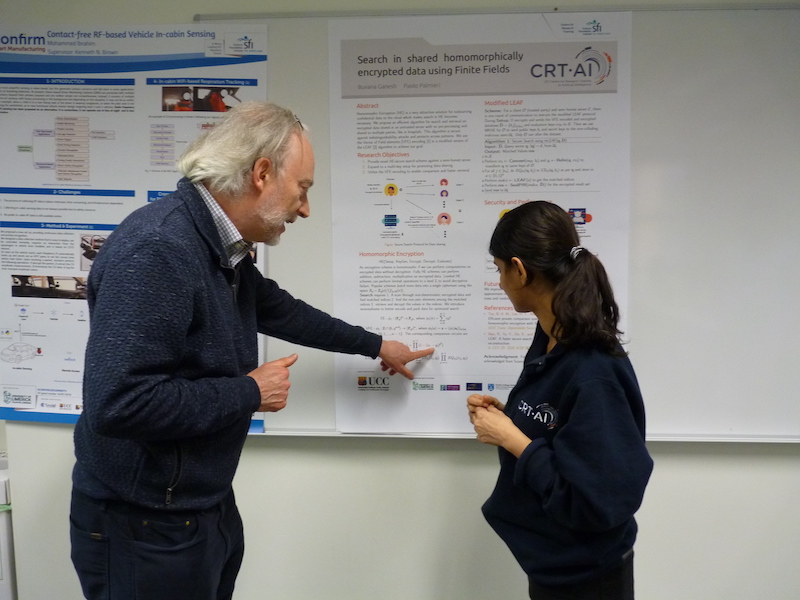
\includegraphics[height=1.88in]{img/phdreview1.JPG} \\

\end{tabular}
\end{figure}

\subsection{Comment and reflect on the relationship (if any) between the department's outreach, engagement, and support activities and issues or opportunities in the student pipeline. This should include comment on how the department recognises staff and student contributions to these activities and monitors the gender balance of those involved.}

The school participates in all
university outreach activities including Open Days 
and careers guidance briefings (Figure~\ref{fig:utzwithkids}). It also hosts
its own initiatives, including  annual information 
evenings, a very popular programme of weekend programming 
classes\footnote{Munster Programming Training (MPT)
\url{https://www.ucc.ie/en/csschools/mpt/}}
and summer camps,\footnote{\url{https://www.ucc.ie/en/csschools/ictsummercamp/}}
 aimed at second-level students, 
in addition to regular school visits 
(Table~\ref{tab:schoolvisits}). All activities are 
tailored to support diversity of undergraduate intake.

\input{tables2/tab_school_visits_18nov}


\begin{figure}[!t]
\caption[Outreach activities at CSIT]{From left to right: Outreach activities at CSIT. Head of School Prof Utz Roedig with potential future students. Visit from transition year students. Munster Programming Training. UCC Open Day.}
\label{fig:utzwithkids}
\begin{tabular}{c !{\quad} c}
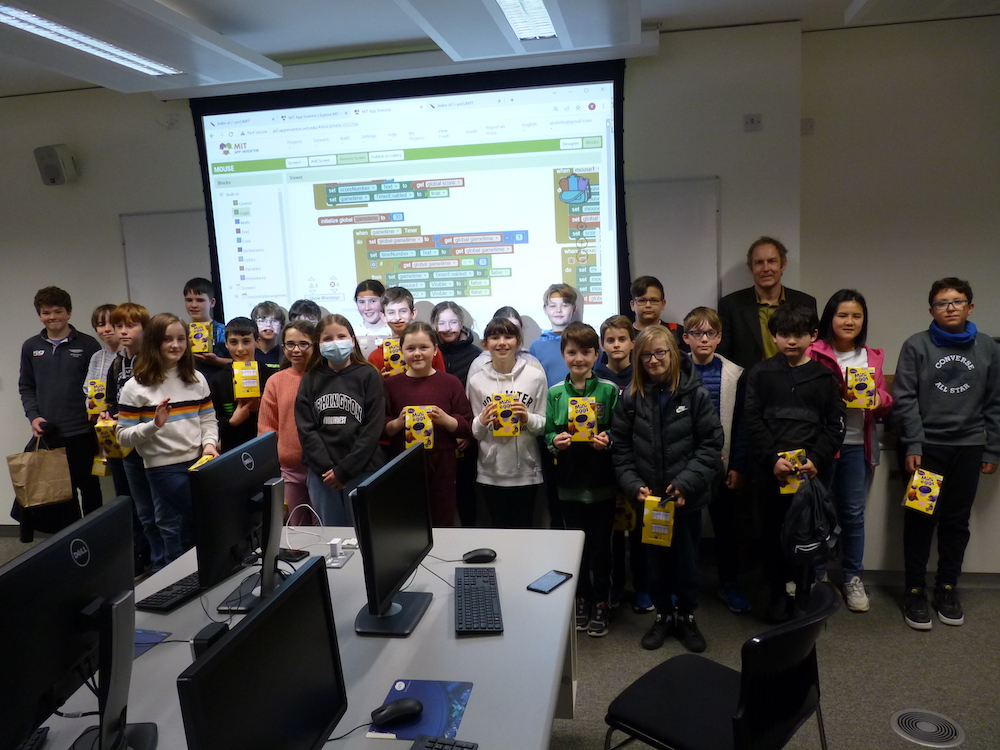
\includegraphics[width=2.85in]{img/utzwithkids.JPG} &
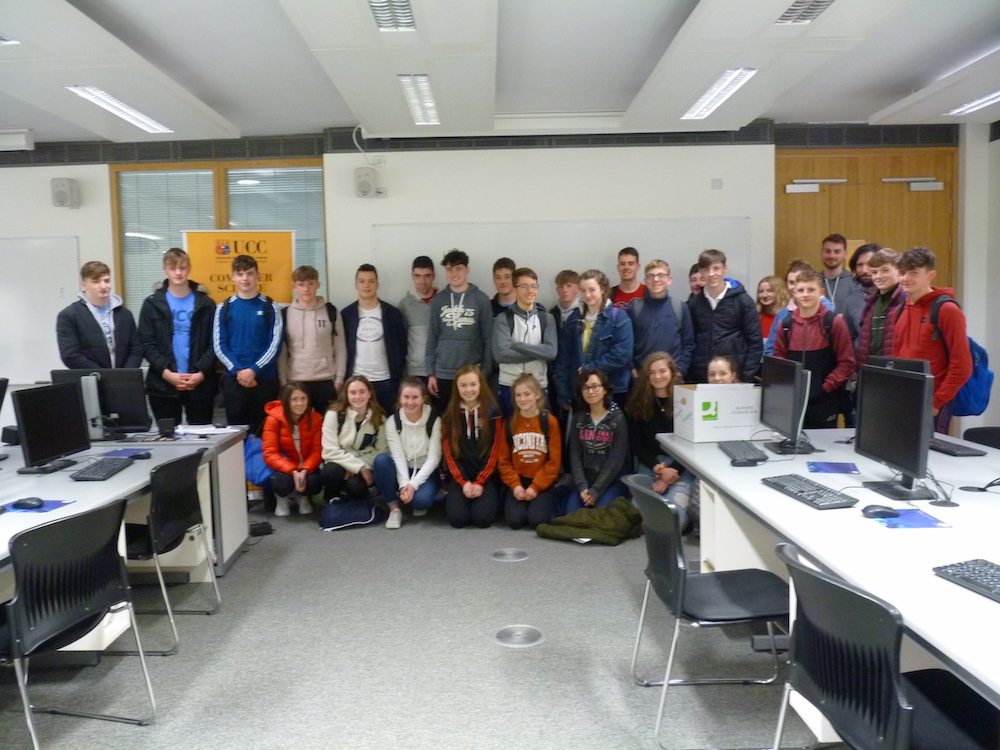
\includegraphics[width=2.85in]{img/futurestudents.JPG} \\
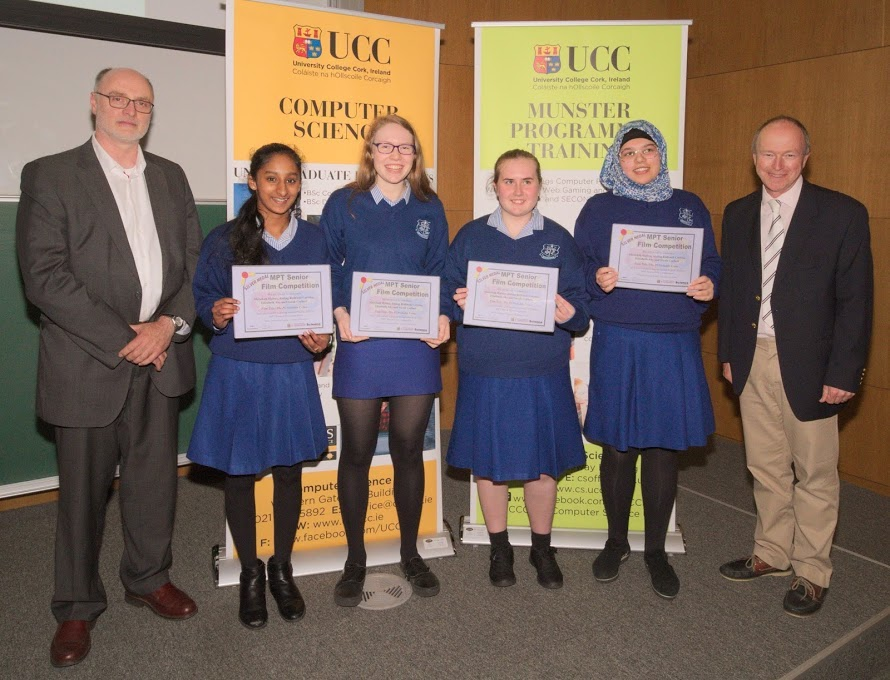
\includegraphics[trim={0 3mm 0 0},clip,width=2.85in]{img/winner_14 mount mercy_1.jpg} &
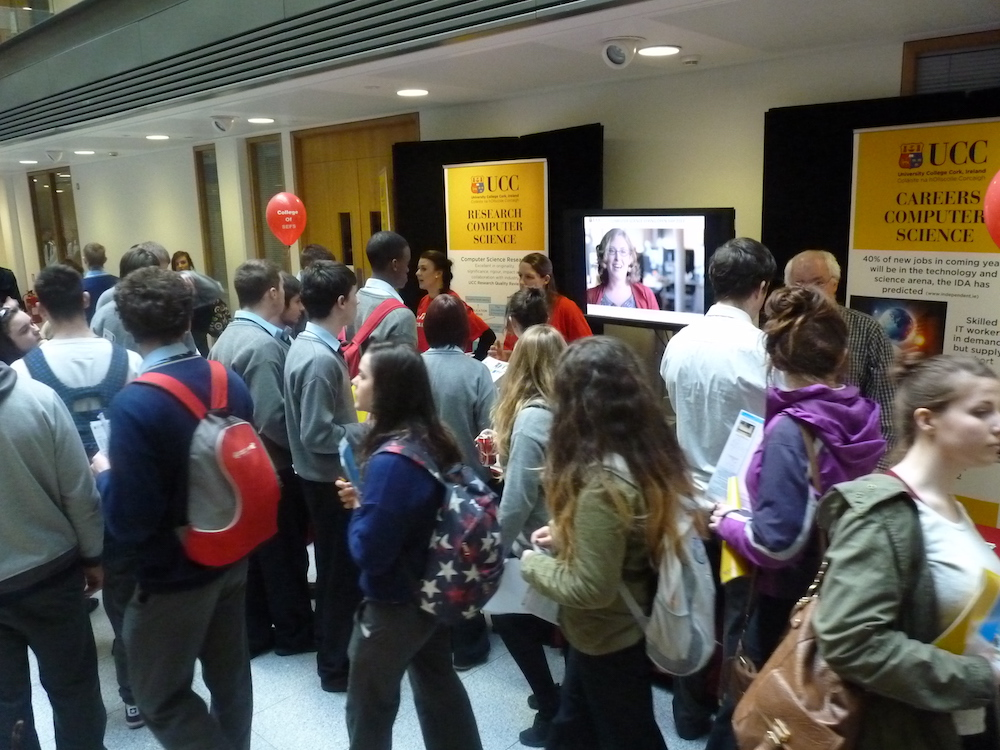
\includegraphics[width=2.85in]{img/openday.JPG} \\

\end{tabular}
\end{figure}

Our existing outreach, marketing and support measures
have evolved in an ad-hoc manner over the years; the 
current AS exercise has highlighted the need for
a comprehensive audit of these activities 
to assess their effectiveness and reflect on how they might 
be reconfigured to address the two key challenges in the 
student pipeline:
\begin{enumerate}[noitemsep]
\item  the under-representation of females in the BScCS and BScDSA 
(Table~\ref{tab:teachingportfolio}); 
\item the lack of female undergraduates who opt to 
progress to graduate research studies.
\end{enumerate}

A survey of current female undergraduates 
(Action~\ref{action:survey:females}) will help inform a 
review of existing marketing and outreach
activities and reconfigure these activities to improve
recruitment of females and to enhance diversity of intake
more generally (Actions~\ref{action:cult:diverseoutreach}
and \ref{action:review:outreach}).
Action~\ref{action:survey:females} will also  diagnose issues
with how the school projects itself to prospective undergraduates.


\begin{actionblock}{\ksspace{}Investigate female perceptions towards
Computer Science and careers}{survey:females}
\actsurveyugfemales
\hfill{
    \hypersetup{hidelinks}
    \hyperlink{b0}{\gotoactionsymbol{}}
}
\end{actionblock}



\begin{actionblock}{\ksspace{}Improve focus on diversity in outreach activities}{cult:diverseoutreach}
\actreviseoutreachpractice
\hfill{
    \hypersetup{hidelinks}
    \hyperlink{b6}{\gotoactionsymbol{}}
}
\end{actionblock}

\begin{actionblock}{\ksspace{}Re-assess and re-configure
existing outreach and support measures}{review:outreach}
\actreviewactivities
\hfill{
    \hypersetup{hidelinks}
    \hyperlink{b2}{\gotoactionsymbol{}}
}
\end{actionblock}



Linking with Action~\hyperlink{act511}{5.1.1}
of UCC's AS Action Plan 2019-2023,\footnote{\url{https://www.ucc.ie/en/media/support/edi/athenaswan/AthenaSWANUCCActionPlan2019-2023.pdf}}
Actions~\ref{action:genderproof:guidelines} 
and \ref{action:boost:visibility} 
will underpin  an overhaul of materials to help reshape recruitment 
materials for future academic, research and PMS vacancies 
(e.g. Action~\ref{action:acad:marketing} and 
Action~\ref{action:pms:matchdescription}).

\begin{UCCaction}{5.1.1}{}\hypertarget{act511}
Revise equality of opportunity statement in recruitment material to reflect a more inclusive, positive and specific commitment to equality principles Develop guidance for writing equality-focused post advertisements, including statements encouraging applications from the underrepresented groups.
\end{UCCaction}


\begin{actionblock}{\ksspace{}Develop gender proofing guidelines
for materials}{genderproof:guidelines}
\actgenderproof
\hfill{
    \hypersetup{hidelinks}
    \hyperlink{b1}{\gotoactionsymbol{}}
}
\end{actionblock}

\begin{actionblock}{\ksspace{}Boost visibility of females}{boost:visibility}
\actboostvisibility
\hfill{
    \hypersetup{hidelinks}
    \hyperlink{b3}{\gotoactionsymbol{}}
}
\end{actionblock}

The recent appointment of a dedicated mentor
has proved effective in improving student experience
for international students. A mentor for female undergraduate students 
will be appointed to offer 
guidance and support (Action~\ref{action:edi:coach}), help coordinate various female-focused 
initiatives,
and encourage female undergraduates to pursue career-enhancing
opportunities e.g., IGNITE entrepreneur incubation 
initiative,\footnote{\url{https://www.ucc.ie/en/ignite/}}
scholarships and internships aimed at  female 
undergraduates (e.g. Huawei, Google), 
participation in events, such as the Irish Programming Olympiad and 
the International Olympiad for Informatics and engagement
with organisations devoted to supporting young women in STEM
such as 
iWish,\footnote{\url{https://www.iwish.ie}}
WiSTEM\footnote{\url{https://www.facebook.com/UCCWiSTEM/}}
and IEEE Women in Engineering (Figure~\ref{fig:olympiad}).


\begin{figure}[!t]
\caption{From top left to bottom right: Irish Programming Olympiad; Huawei Scholarships; Google sponsorship of Irish Collegiate Programming Competition; UCC Quercus Talented Students Programme}
\label{fig:olympiad}
\begin{tabular}{c !{\quad} c}
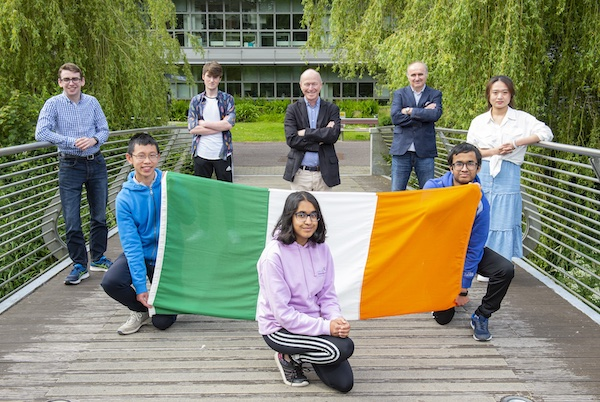
\includegraphics[height=2.035in]{img/olympiad.jpg} &
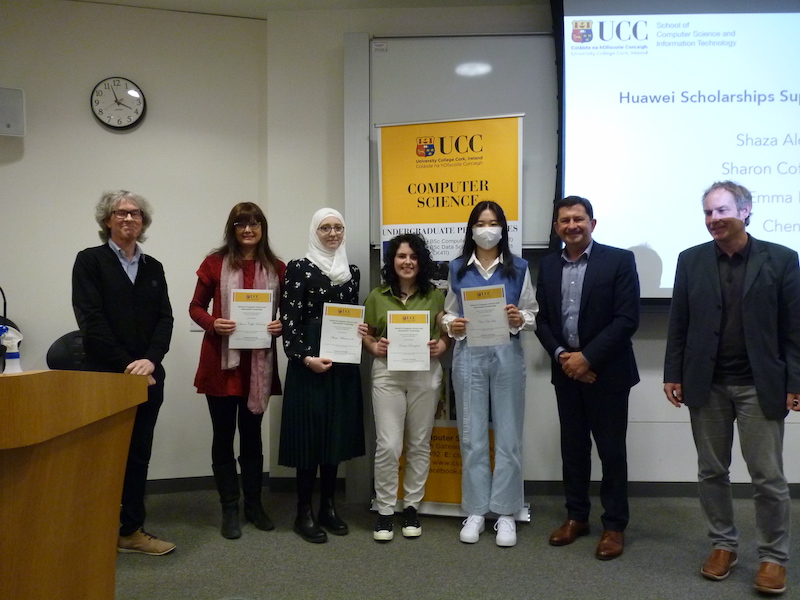
\includegraphics[height=2.035in]{img/huawei.JPG} \\
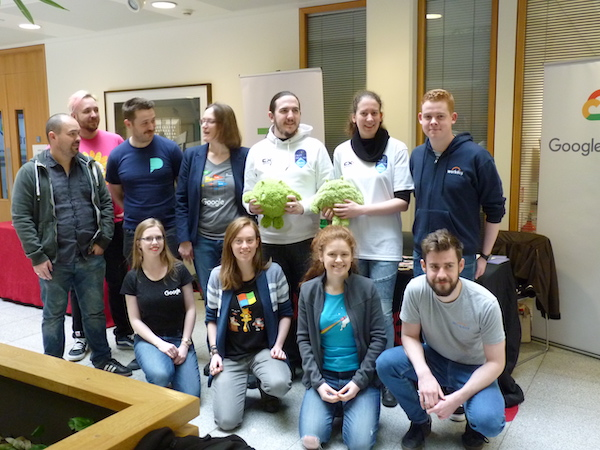
\includegraphics[trim={0 0mm 0 17mm},clip,height=2.035in]{img/google.JPG} &
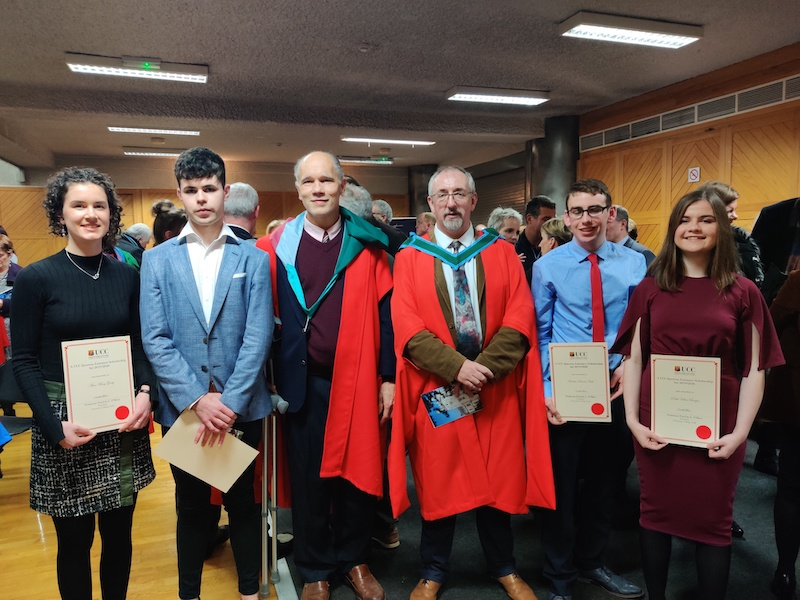
\includegraphics[height=2.035in]{img/quercus.jpg} \\

\end{tabular}
\end{figure}

\begin{actionblock}{\ksspace{}Appoint mentor for female undergraduates}{edi:coach}
\actappointmentor
\hfill{
    \hypersetup{hidelinks}
    \hyperlink{b4}{\gotoactionsymbol{}}
}
\end{actionblock}

Encouraging female undergraduates to consider a research career 
will be challenging given economic and career 
factors explored in Subsection~\ref{subsec:academic_research}, 
however,  research internship opportunities may help nurture interest (Action~\ref{action:enrich:opportunities}). 

%\todo{JPM changed name of action and preceeding text}
\begin{actionblock}{\ksspace{}Internship opportunities for female undergraduates}{enrich:opportunities}
\actenrichopportunities
\hfill{
    \hypersetup{hidelinks}
    \hyperlink{b5}{\gotoactionsymbol{}}
}
\end{actionblock}

The school aims for gender balanced  representation (both staff and students) at all outreach activities.


\subsection{Provide data for academic and research staff by gender and grade. Analyse and benchmark the career pipeline.}
\label{subsec:academic_research}




Table~\ref{tab:acresstaff} demonstrates that the gender imbalance is stark for both academic and researchers
and at senior levels: there is no female at Senior Postdoctoral 
level or above nor at \ac{SL} level or above. 

Table~\ref{tab:academic_benchmark} compares CSIT's academic
staff profile with that of two peer institutions, \ac{UCD} 
and \ac{TCD}.
The percentage of female academics at CSIT is 9\%, 
compared with 16\% at UCD and 29\% at TCD. 
CSIT has no females at \ac{SL}
level or above, compared with six out of 58 at UCD and five 
out of 59 at TCD. \ac{HESA} data  (2019-20 ICTS) from the 
UK indicates 16\% professors in \ac{CS} are females, 
and 22\% of all research and academic staff excluding professors.

% Modified KH on 18 Nov to swap MF cols.

\begin{tabbox}[12cm]{!t}
\caption{CSIT academics and researchers (2020)}
\label{tab:acresstaff}
\footnotesize 

      
\begin{tabular}{p{4cm}
                C{1cm}
                C{1cm}
                c
                p{0.7cm}
                C{1cm}
                C{1cm}
                c
                !{\qquad}
                C{1cm}}
\toprule 
%\multicolumn{7}{c}{\bfseries Academics and Researchers (2020)}\\ \hline
  & \multicolumn{3}{c}{Permanent/CID} && \multicolumn{3}{c}{Fixed-Term}\\
  \cmidrule{2-4}\cmidrule{6-8}
%  Grade & {F} & {M} & \%F && {F} & {M} & \%F\\
  Grade & {M} & {F} & \%F && {M} & {F} & \%F & Total\\
  \midrule 

  Academics \\
  \midrule   
  Professor& 4& -& -&&- &- &- & 4\\
  \hdashline   
  Professor (Scale 2) &4 & -&- &&- &- &- &4\\
  \hdashline   
  Senior Lecturer &5& -&- &&- &- &- & 5\\
  \hdashline 
  %Lecturer (above bar)&1 &14 &7\% &&- & 1&- \\
  Lecturer (above bar)&14 &1 &6.7\% &&1 & -&- & 16\\
  \hdashline 
  %Lecturer (below bar)&1 &-& 100\% && 1&2 & 33\%\\
  Lecturer (below bar)&- &1& 100\% && 2&1 & 33\% & 4\\ 
  \midrule 
  Subtotal academics & 27 & 2 & 6.9\% & & 3 & 1 & 25\% & 33\\
\midrule 
%\addlinespace
%\midrule 
Research staff\textsuperscript{1} \\
\midrule 
 %Senior Research Fellow&- &- &- &&- & 1&-\\
 Senior Research Fellow&- &- &- &&1 & -&- & 1\\
 \hdashline 
 %Research Fellow &- & -&- &&- &3 &-\\
 Research Fellow &- & -&- &&3 &- &- & 3\\
 \hdashline 
 %Senior Postdoc &- &- &- &&- &4 &- \\
 Senior Postdoc &- &- &- &&4 &- &- & 4\\
 \hdashline 
 %Postdoc & - &- &- &&3 &10 & 23\%\\
 Postdoc & - &- &- &&10 &3 & 23\% & 13\\
 \hdashline 
 %Research Assistant &- &- &- && 1&1 & 50\%\\
 Research Assistant &- &- &- && 1&1 & 50\% & 2\\
 \midrule 
 Subtotal researchers & - & - & - & & 19 & 4 & 17.4\% & 23\\
\bottomrule 
\end{tabular}
\\[2mm]
{\sffamily \textsuperscript{1}Research staff are hired on fixed-term contracts only.}


\end{tabbox}


%
% Have tried to replicate your table style using 
% 'tab_taught_programmes as a model.
%

% Material from here to 'preamble' marker below copied
% verbatim from model aprt from caption and label.
%
\begin{tabbox}{!h}


\caption{Academic staff by grade and gender benchmarked against
peer institutions}
\label{tab:academic_benchmark}
\footnotesize 

\sisetup{
    group-digits=all,
    group-minimum-digits=4,
    mode=text,
    reset-text-series = false, 
    text-series-to-math = true,
    reset-text-family=false, 
    text-family-to-math=true
}
% 'preamble ends here'

                
\begin{tabular}{p{7.3cm}
                C{1cm}C{1cm}
                p{.5cm}
                C{1cm}C{1cm}
                p{.5cm}
                C{1cm}C{1cm}
               }
\toprule
&
\multicolumn{2}{c}{\textmd{UCC}}&&
\multicolumn{2}{c}{\textmd{UCD}}&&
\multicolumn{2}{c}{\textmd{TCD}}\\
\cmidrule(l){2-3}\cmidrule(l){5-6}\cmidrule(l){8-9}
Grade & M & F && M & F && M & F\\
\midrule 
Professors&
8 & - & &7 & 3 && 10 & 3\\
\hdashline 
Senior Lecturer &
5 & - & &17 & 3 && 9 & 2\\
\hdashline 
Lecturer&
17 & 3 && 25 & 3 && 23 & 12\\
\midrule
Subtotal Senior Lecturer or above&
13 & - && 24 & 6 && 19 & 5\\
\hdashline 
Total&
30 & 3 && 49 & 9 && 42 & 17\\

% Material from here on copied verbatim from model.
\bottomrule 

\end{tabular}
\vspace{2mm}\\
{\sffamily

Sources:
UCD, School of Computer Science (\url{www.ucd.ie/cs}).
TCD, School of Computer Science and Statistics, (\url{www.scss.tcd.ie}); numbers include some statisticians.
}

\end{tabbox}

% Notes:
% Scraped from webpage except
% Andrea and Harry added



CSIT's academic gender profile is largely a reflection of an
uneven recruitment pattern over decades. An expansion of
staff numbers in the 1990s and early 2000s was followed by 
a prolonged  hiring drought, which locked in a historical 
all-male imbalance. Prior to 2017, when our first female colleague 
was recruited, no permanent academic appointment
had been made since 2004.
% Note 2017: AOD, AZ, KJS & PP joined
% 2004: GP joined and none in intervening period.


\pagebreak 
However, since 2017 CSIT has filled 13 academic posts 
(nine male and four female), two of whom (one male, one female)
have since resigned to take up posts in their home country.
%male: KJS, AZ, PP, AA, UR, DP, HC, AV, Harry
%females: AOD, LC,  LM, RM
While this is a step in the right direction, the school realises that 
much work remains to be done to achieve a healthy gender balance, and
%The healthier gender balance evident in recent hires is a positive development and a trend 
will  
adopt gender-positive recruitment measures described in
Section~\ref{sec:academic}
(e.g. Actions~\ref{action:acad:marketing}--\ref{action:acad:cvgaps}).

In the years up to 2027, 12 staff (nine academic, three administrators) are
expected to reach the normal retirement age. Some additional new posts
are also expected based on increasing student numbers. % from new programmes.
This significant number of openings presents an opportunity to approach 
recruitment in a strategic manner, not least to further 
improve gender balance. 



\begin{figbox}{!t}
    \caption[Career pipeline: gender distribution across academic levels of seniority]{Career pipeline: gender distribution across academic levels of seniority, from undergraduate students to Senior Lecturer (SL) and above (2020)}
    \label{fig:pipeline}
    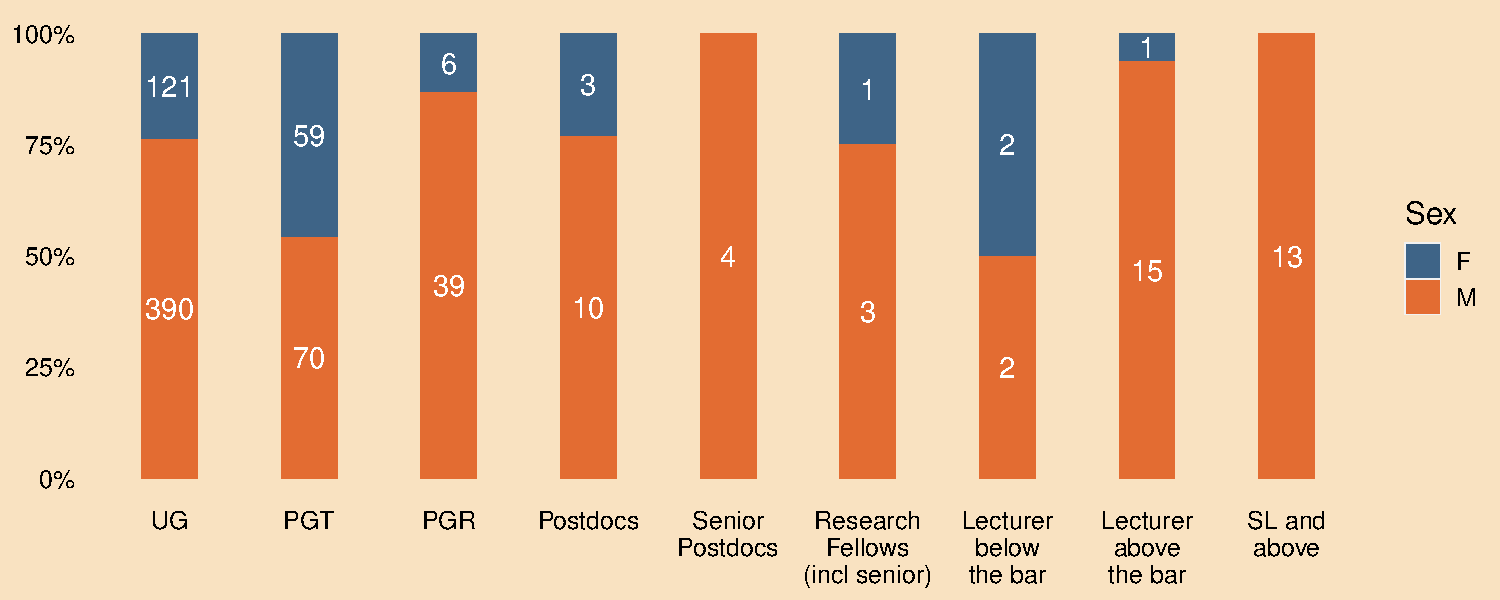
\includegraphics[trim={0 2mm 0 0},clip,width=5.7in]{fig/pipeline.pdf}
\end{figbox}

% \todo{[KJS: Insert figure "The career pipeline"; Tweak to include 
% undergraduates (24\%) and taught postgraduate (46\%) bars.
% See email of 2 Aug 2022.]}

Figure~\ref{fig:pipeline} depicts the career pipeline, showing the
the percentage of females at different career levels from 
undergraduates to professors. 
The ``pipeline'' metaphor can result in an over-focus
on flow from beginning to end, potentially downplaying important 
inward flows at various stages. For example, very few Irish 
undergraduates progress to masters programmes and fewer still
to research studies. 
The healthy numbers and gender balance in our postgraduate programmes 
is largely due to non-EU students. 
%entering at masters or PhD level.
These inward flows are very welcome but camouflage the dearth of female 
undergraduates progressing through PhD and onward to research and
academic careers.

The tapering proportion of females from undergraduates to lecturers to 
senior academics is a global phenomenon in \ac{CS}, but the 
complete lack of females in senior grades at UCC is an outlier even 
within our traditionally male-dominated discipline. 
The greatest choke points appear to be:


\begin{enumerate}[noitemsep]
    \item From undergraduate to research postgraduate
    \item From research roles to academic posts
    \item From Lecturer to \ac{SL} and beyond
\end{enumerate}


Employment prospects for Irish 
computing graduates are buoyant and, unlike other STEM disciplines, 
further postgraduate study is not required for career opportunities
in industry. 

Factors deterring research students and postdocs from pursuing 
academic careers are explored further in 
Section~\ref{sec:academic}. 
Poor PhD stipends (currently at \texteuro{}18,500 p.a.) and low
pay for postdoctoral positions relative to attractive industry salaries 
is one factor. 
Starting salaries on offer to talented 
graduates can be a multiple of the PhD stipend. 
Uncertainties surrounding  securing academic 
positions and promotional opportunities thereafter is another. 


As noted, CSIT has no female academics at \ac{SL}
rank or above, so the Lecturer/\ac{SL} boundary represents
a significant choke point. \label{slboundary}
At UCC academics can attain a senior grade 
either through promotion or direct appointment to an advertised 
position. Promotion criteria and processes at UCC are 
dictated entirely 
by the university and the school has had very limited success with 
promotions over the years.
In the past twenty years, there have been six academic
promotions in all (none since 2014; no females as CSIT did not 
have any female academics until 2017), 
but only three from Lecturer to 
\ac{SL} (most recently in 2008).
In the most recent round (2018-2019), only two 
Lecturers applied for promotion to \ac{SL}; neither was successful (Table~\ref{tab:promotion2sl}).  
If promotions are to contribute to improving gender balance at senior 
levels, 
the school will proactively support colleagues, particularly
females, in navigating UCC's promotion scheme successfully (Action~\ref{action:acad:mentoring}). 

Section~\ref{sec:academic} explores staff experiences
and perception with recruitment and  promotions and proposes
some actions to help improve the gender balance over time. 





\subsection{Provide data for professional, managerial and support staff by gender and grade. Analyse representation, benchmarking where possible.}


% \khcomment{TCD website may allow benchmarking for sysadmin staff}

Table~\ref{tab:pmsstaff} gives an overview of the numbers of \ac{PMS} staff. UCC  classifies
staff in  \ac{CSSS} as ``administrative'' rather than 
``technical.''

% Modified KH on 18 Nov to swap MF cols.

\begin{tabbox}{!th}
\caption[Professional, Managerial, and Support staff (2020)]{Professional, Managerial, and Support staff (2020) (includes core and research IT support staff)}
\label{tab:pmsstaff}
\footnotesize       

\sisetup{
    group-digits=all,
    group-minimum-digits=4,
    table-format=2.1,
    mode=text,
    reset-text-series = false, 
    text-series-to-math = true,
    reset-text-family=false, 
    text-family-to-math=true
}
\begin{tabular}{P{3.5cm}  
                p{4.2cm} 
                S[table-format=2.1]
                !{\quad}
                S[table-format=2.1]
                !{\quad}
                S[table-format=3.0\%]
                p{0.5cm}
                S[table-format=2.1]
                !{\quad}
                S[table-format=2.0\%]
                !{\quad}
                S[table-format=2.0]
                p{0.5cm}
                S[table-format=2.0]}
\toprule 

 & & \multicolumn{3}{c}{Permanent/CID}& & \multicolumn{3}{c}{Fixed-Term}\\
 \cmidrule{3-5}\cmidrule{7-9}

 & &{M} & {F} & \%F & & {M} & {F} & \%F && {Total}\\
\midrule 

Office& Grades 5+ (Admin) &{-}  & 2 &100\% &&{-} &{-} &{-}  && 2\\
 
\cdashline{2-11}
& Senior Executive Assistant & 1&1 &50\% &&{-} &{-} &{-}  && 2\\
\cdashline{2-11}
& Executive Assistant & {-} &2 &100\% &&{-} &{-} &{-}  & &2\\ 

\hdashline
Computer Science Systems Support & Grades 5+ (IT) &5 & {-}  &{-}  & &{-} &{-} &{-}  && 5\\  
\hdashline
Research
& Support staff& {-} &{-}  &{-}  &&7 &7 &50\% && 14\\
\midrule
Total & & 6 & 5 & 46\% & & 7 & 7 & 50\% && 25\\
\bottomrule 
\end{tabular}
\sffamily

\end{tabbox}


Among those in administrative roles in the school's office, 
females predominate; mirroring the situation within the university.
The school's core IT staff are exclusively male. This gender
pattern for administrative and IT roles is replicated among the 
research support staff.
Section~\ref{sec:pms} explores this issue in greater depth 
and presents actions to move the school on a more gender-balanced
trajectory for PMS staff
(e.g. Action
~\ref{action:pms:matchdescription}).

By way of comparison, TCD's webpage currently lists 24 administrative 
staff (21 female, 3 male), nine IT support staff (three female, six
male) and six staff classified as technicians (all male).



\subsection{Provide data on staff on fixed-term contracts, contracts of indefinite duration/permanent contracts, and hourly-paid contracts by gender and staff category. Outline instances where fixed-term and hourly-paid contract types are used. This should include comment on:}
\instr{
\begin{itemize}
    \item whether or not numbers of fixed-term/hourly-paid contracts are representative of a typical year; 
    \item the rationale for the use of short-term contracts;
    \item the extent to which hourly-paid staff contribute to the teaching of core modules and/or services.
\end{itemize}
}

Table~\ref{tab:fthpstaff} summarises CSIT staff by category, contract 
type and gender for 2020.

% Modified KH on 18 Nov to swap MF columns.

\begin{tabbox}{!th}

\caption{CSIT staff by category, contract type and gender
(2020)}
\label{tab:fthpstaff}
\footnotesize 

      
\begin{tabular}{p{3cm}
                C{1cm}
                C{1cm}
                C{1cm}
                p{0.5cm}
                C{1cm}
                C{1cm}
                C{1cm}
                p{0.5cm}
                C{1cm}
                C{1cm}
                C{1cm}
                p{0.5cm}
                C{1cm}}
\toprule 
%\multicolumn{7}{c}{\bfseries Academics and Researchers (2020)}\\ \hline
  & \multicolumn{3}{c}{Permanent/CID} && \multicolumn{3}{c}{Fixed-Term} && \multicolumn{3}{c}{Hourly-Paid}\\
  \cmidrule{2-4}\cmidrule{6-8}\cmidrule{10-12}
%  Category  & {F} & {M} & \%F && {F} & {M} & \%F && {F} & {M} & \%F\\
  Category  & {M} & {F} & \%F && {M} & {F} & \%F && {M} & {F} & \%F && {Total}\\
  \midrule 


  Academic&27 &2 &7\% && 2 & 2 & 50\% && 1 &- & 0\% && 34\textsuperscript{1}\\
  \hdashline 

  Researchers&- &- &- &&19 & 4 & 17\% && - &- &- && 23\\
  \hdashline 

  PMS &6 &5  & 45\% & & 7 & 7 & 50\% & & - & - &- && 25\\
  \midrule
  Total & 33 & 7 & 17.5\% && 28 & 13 & 32\%  & & 1 & - & 0\% && 82\\
\bottomrule 
\end{tabular}
{
\vspace{2mm}\\
\sffamily
\textsuperscript{1}Hourly-paid academic staff were not included in earlier tables.
Some fixed-term PMS staff listed here have 
permanent/CID posts but are operating at a higher grade
in research support roles.
}
\end{tabbox}


\subsubsection{Comment on whether or not numbers of fixed-term/hourly-paid contracts are representative of a typical year}

The  pattern seen in Table~\ref{tab:fthpstaff}
is  typical of recent years. Hourly-paid contracts are 
never used for research or PMS roles and only rarely for 
academics, as noted below.


\subsubsection{Comment on the rationale for the use of short-term contracts}
\label{rationalecontracts}

Short-term academic contracts (typically one year) are used 
to cover temporary vacancies in permanent posts arising from
maternity cover and retirements. Also posts tied to new programmes are often
sanctioned on a fixed-term basis initially.
%, but the school
%actively lobbies for these to be converted into permanent
%posts.
% DT: Fixed terms 2020: LAB={RM}; LBB = {LM. JQ}
Three of the fixed-term academic shown in 
Table~\ref{tab:fthpstaff} have subsequently received 
permanent positions, two of whom are female.



Research activity is wholly dependent on the flow of research 
funding which is inherently impermanent and so all researchers 
are on fixed-term contracts. A number of those in research 
administration or research IT support roles have core
permanent/\ac{CID} positions, some appointed to a 
higher-grade from research funds.

\subsubsection{Comment on the extent to which hourly-paid staff contribute to the teaching of core modules and/or services}

Hourly paid staff are mainly students
employed on a part-time basis as laboratory demonstrators or tutors for
undergraduate modules. The amount of such work varies by year; 
in 2019-20, for example, we had 65 hourly paid staff: 54 male and 11 female (17\%), which is below the percentage of 
female undergraduate and taught postgraduates.

A handful of modules (3\%) are covered by hourly-paid part-time lecturers---generally postdocs seeking teaching experience.





